\documentclass[twoside]{book}

% Packages required by doxygen
\usepackage{fixltx2e}
\usepackage{calc}
\usepackage{doxygen}
\usepackage{graphicx}
\usepackage[utf8]{inputenc}
\usepackage{makeidx}
\usepackage{multicol}
\usepackage{multirow}
\PassOptionsToPackage{warn}{textcomp}
\usepackage{textcomp}
\usepackage[nointegrals]{wasysym}
\usepackage[table]{xcolor}

% Font selection
\usepackage[T1]{fontenc}
\usepackage{mathptmx}
\usepackage[scaled=.90]{helvet}
\usepackage{courier}
\usepackage{amssymb}
\usepackage{sectsty}
\renewcommand{\familydefault}{\sfdefault}
\allsectionsfont{%
  \fontseries{bc}\selectfont%
  \color{darkgray}%
}
\renewcommand{\DoxyLabelFont}{%
  \fontseries{bc}\selectfont%
  \color{darkgray}%
}
\newcommand{\+}{\discretionary{\mbox{\scriptsize$\hookleftarrow$}}{}{}}

% Page & text layout
\usepackage{geometry}
\geometry{%
  a4paper,%
  top=2.5cm,%
  bottom=2.5cm,%
  left=2.5cm,%
  right=2.5cm%
}
\tolerance=750
\hfuzz=15pt
\hbadness=750
\setlength{\emergencystretch}{15pt}
\setlength{\parindent}{0cm}
\setlength{\parskip}{0.2cm}
\makeatletter
\renewcommand{\paragraph}{%
  \@startsection{paragraph}{4}{0ex}{-1.0ex}{1.0ex}{%
    \normalfont\normalsize\bfseries\SS@parafont%
  }%
}
\renewcommand{\subparagraph}{%
  \@startsection{subparagraph}{5}{0ex}{-1.0ex}{1.0ex}{%
    \normalfont\normalsize\bfseries\SS@subparafont%
  }%
}
\makeatother

% Headers & footers
\usepackage{fancyhdr}
\pagestyle{fancyplain}
\fancyhead[LE]{\fancyplain{}{\bfseries\thepage}}
\fancyhead[CE]{\fancyplain{}{}}
\fancyhead[RE]{\fancyplain{}{\bfseries\leftmark}}
\fancyhead[LO]{\fancyplain{}{\bfseries\rightmark}}
\fancyhead[CO]{\fancyplain{}{}}
\fancyhead[RO]{\fancyplain{}{\bfseries\thepage}}
\fancyfoot[LE]{\fancyplain{}{}}
\fancyfoot[CE]{\fancyplain{}{}}
\fancyfoot[RE]{\fancyplain{}{\bfseries\scriptsize Generated on Mon Mar 6 2017 15\+:57\+:21 for Reconocimiento de genes en secuencias de A\+D\+N utilizando el algoritmo Aho-\/\+Corasick by Doxygen }}
\fancyfoot[LO]{\fancyplain{}{\bfseries\scriptsize Generated on Mon Mar 6 2017 15\+:57\+:21 for Reconocimiento de genes en secuencias de A\+D\+N utilizando el algoritmo Aho-\/\+Corasick by Doxygen }}
\fancyfoot[CO]{\fancyplain{}{}}
\fancyfoot[RO]{\fancyplain{}{}}
\renewcommand{\footrulewidth}{0.4pt}
\renewcommand{\chaptermark}[1]{%
  \markboth{#1}{}%
}
\renewcommand{\sectionmark}[1]{%
  \markright{\thesection\ #1}%
}

% Indices & bibliography
\usepackage{natbib}
\usepackage[titles]{tocloft}
\setcounter{tocdepth}{3}
\setcounter{secnumdepth}{5}
\makeindex

% Hyperlinks (required, but should be loaded last)
\usepackage{ifpdf}
\ifpdf
  \usepackage[pdftex,pagebackref=true]{hyperref}
\else
  \usepackage[ps2pdf,pagebackref=true]{hyperref}
\fi
\hypersetup{%
  colorlinks=true,%
  linkcolor=blue,%
  citecolor=blue,%
  unicode%
}

% Custom commands
\newcommand{\clearemptydoublepage}{%
  \newpage{\pagestyle{empty}\cleardoublepage}%
}


%===== C O N T E N T S =====

\begin{document}

% Titlepage & ToC
\hypersetup{pageanchor=false,
             bookmarks=true,
             bookmarksnumbered=true,
             pdfencoding=unicode
            }
\pagenumbering{roman}
\begin{titlepage}
\vspace*{7cm}
\begin{center}%
{\Large Reconocimiento de genes en secuencias de A\+D\+N utilizando el algoritmo Aho-\/\+Corasick \\[1ex]\large V1.\+0 }\\
\vspace*{1cm}
{\large Generated by Doxygen 1.8.8}\\
\vspace*{0.5cm}
{\small Mon Mar 6 2017 15:57:21}\\
\end{center}
\end{titlepage}
\clearemptydoublepage
\tableofcontents
\clearemptydoublepage
\pagenumbering{arabic}
\hypersetup{pageanchor=true}

%--- Begin generated contents ---
\chapter{Hierarchical Index}
\section{Class Hierarchy}
This inheritance list is sorted roughly, but not completely, alphabetically\+:\begin{DoxyCompactList}
\item \contentsline{section}{B\+S\+T$<$ Data $>$}{\pageref{class_b_s_t}}{}
\item \contentsline{section}{Cell$<$ D $>$}{\pageref{class_cell}}{}
\item \contentsline{section}{Cell$<$ Edge$<$ Data $>$ $>$}{\pageref{class_cell}}{}
\item \contentsline{section}{Cell$<$ Node$<$ D $>$ $>$}{\pageref{class_cell}}{}
\item \contentsline{section}{Cell$<$ Node$<$ Data $>$ $>$}{\pageref{class_cell}}{}
\item \contentsline{section}{Data$<$ D $>$}{\pageref{class_data}}{}
\item \contentsline{section}{Edge$<$ D $>$}{\pageref{class_edge}}{}
\item \contentsline{section}{Edge$<$ Data $>$}{\pageref{class_edge}}{}
\item \contentsline{section}{Graph$<$ Data $>$}{\pageref{class_graph}}{}
\item \contentsline{section}{Graph\+With\+Array}{\pageref{class_graph_with_array}}{}
\item \contentsline{section}{List$<$ D, P $>$}{\pageref{class_list}}{}
\begin{DoxyCompactList}
\item \contentsline{section}{List\+With\+Array$<$ D, P $>$}{\pageref{class_list_with_array}}{}
\item \contentsline{section}{List\+With\+Pointer$<$ D, P $>$}{\pageref{class_list_with_pointer}}{}
\end{DoxyCompactList}
\item \contentsline{section}{List$<$ Edge$<$ Data $>$, Cell$<$ Edge$<$ Data $>$ $>$ $\ast$ $>$}{\pageref{class_list}}{}
\begin{DoxyCompactList}
\item \contentsline{section}{List\+With\+Pointer$<$ Edge$<$ Data $>$, Cell$<$ Edge$<$ Data $>$ $>$ $\ast$ $>$}{\pageref{class_list_with_pointer}}{}
\end{DoxyCompactList}
\item \contentsline{section}{List$<$ N\+O\+D\+E, int $>$}{\pageref{class_list}}{}
\item \contentsline{section}{List$<$ Node$<$ D $>$, Cell$<$ Node$<$ D $>$ $>$ $\ast$ $>$}{\pageref{class_list}}{}
\begin{DoxyCompactList}
\item \contentsline{section}{List\+With\+Pointer$<$ Node$<$ D $>$, Cell$<$ Node$<$ D $>$ $>$ $\ast$ $>$}{\pageref{class_list_with_pointer}}{}
\end{DoxyCompactList}
\item \contentsline{section}{List$<$ Node$<$ Data $>$, Cell$<$ Node$<$ Data $>$ $>$ $\ast$ $>$}{\pageref{class_list}}{}
\begin{DoxyCompactList}
\item \contentsline{section}{List\+With\+Pointer$<$ Node$<$ Data $>$, Cell$<$ Node$<$ Data $>$ $>$ $\ast$ $>$}{\pageref{class_list_with_pointer}}{}
\end{DoxyCompactList}
\item \contentsline{section}{My\+Data$<$ D $>$}{\pageref{class_my_data}}{}
\item \contentsline{section}{Node$<$ D $>$}{\pageref{class_node}}{}
\item \contentsline{section}{Node$<$ Data $>$}{\pageref{class_node}}{}
\end{DoxyCompactList}

\chapter{Class Index}
\section{Class List}
Here are the classes, structs, unions and interfaces with brief descriptions\+:\begin{DoxyCompactList}
\item\contentsline{section}{\hyperlink{class_d_n_acompare}{D\+N\+Acompare} }{\pageref{class_d_n_acompare}}{}
\item\contentsline{section}{\hyperlink{class_graph_aho_corasick}{Graph\+Aho\+Corasick} }{\pageref{class_graph_aho_corasick}}{}
\item\contentsline{section}{\hyperlink{class_list}{List$<$ D, P $>$} \\*Libreria que genera un template de una clase abstracta list }{\pageref{class_list}}{}
\item\contentsline{section}{\hyperlink{class_list_with_array}{List\+With\+Array$<$ D, P $>$} \\*Libreria que genera un template de una clase \hyperlink{class_list_with_array}{List\+With\+Array} (lista implementada con arreglos) que hereda de la clase \hyperlink{class_list}{List} y que toma un tipo de dato para los datos contenidos en la lista (D) y otro para los indices de las misma (P) }{\pageref{class_list_with_array}}{}
\item\contentsline{section}{\hyperlink{class_stade}{Stade} }{\pageref{class_stade}}{}
\item\contentsline{section}{\hyperlink{class_stade_suc}{Stade\+Suc} }{\pageref{class_stade_suc}}{}
\end{DoxyCompactList}

\chapter{File Index}
\section{File List}
Here is a list of all files with brief descriptions\+:\begin{DoxyCompactList}
\item\contentsline{section}{include/\hyperlink{_cell_8h}{Cell.\+h} }{\pageref{_cell_8h}}{}
\item\contentsline{section}{include/\hyperlink{_list_8h}{List.\+h} }{\pageref{_list_8h}}{}
\item\contentsline{section}{include/\hyperlink{_list_with_array_8h}{List\+With\+Array.\+h} }{\pageref{_list_with_array_8h}}{}
\item\contentsline{section}{include/\hyperlink{_list_with_pointer_8h}{List\+With\+Pointer.\+h} }{\pageref{_list_with_pointer_8h}}{}
\item\contentsline{section}{include/\hyperlink{_queue_8h}{Queue.\+h} }{\pageref{_queue_8h}}{}
\item\contentsline{section}{include/\hyperlink{_stack_8h}{Stack.\+h} }{\pageref{_stack_8h}}{}
\item\contentsline{section}{src/\hyperlink{main_8cpp}{main.\+cpp} }{\pageref{main_8cpp}}{}
\end{DoxyCompactList}

\chapter{Class Documentation}
\hypertarget{class_d_n_acompare}{\section{D\+N\+Acompare Class Reference}
\label{class_d_n_acompare}\index{D\+N\+Acompare@{D\+N\+Acompare}}
}


{\ttfamily \#include $<$D\+N\+Acompare.\+h$>$}

\subsection*{Public Member Functions}
\begin{DoxyCompactItemize}
\item 
\hyperlink{class_d_n_acompare_afc7ea1cba3a91cdf7d6130c73461ce7c}{D\+N\+Acompare} ()
\begin{DoxyCompactList}\small\item\em Constructor de la clase \hyperlink{class_d_n_acompare}{D\+N\+Acompare}. \end{DoxyCompactList}\item 
\hyperlink{class_d_n_acompare_a1fdd0f41d40101045885825ebd9849e9}{D\+N\+Acompare} (string dictionary, string string\+X, string $\ast$words, int percentage, int count\+Words)
\begin{DoxyCompactList}\small\item\em Constructor sobrecargado de la clase \hyperlink{class_d_n_acompare}{D\+N\+Acompare}. \end{DoxyCompactList}\item 
\hyperlink{class_d_n_acompare_adff43389b52e963817bdb08076ce72be}{$\sim$\+D\+N\+Acompare} ()
\begin{DoxyCompactList}\small\item\em Destructor de la clase \hyperlink{class_d_n_acompare}{D\+N\+Acompare}. \end{DoxyCompactList}\item 
int \hyperlink{class_d_n_acompare_a8faa784e087dabfbbb29faa2c9ce0933}{count\+Stades} (string $\ast$sequences)
\begin{DoxyCompactList}\small\item\em Metodo que cuenta la longitud de las palabras para deteminar cuantos estados existen. \end{DoxyCompactList}\item 
string \hyperlink{class_d_n_acompare_ad6944ef2736f6cfcaeec7f07ea174b7c}{get\+Dicc} ()
\begin{DoxyCompactList}\small\item\em Metodo get del atributo dicc. \end{DoxyCompactList}\item 
int \hyperlink{class_d_n_acompare_a5c2ec87d4157c3db16cdb775d0cbf68b}{get\+Num\+Words} ()
\begin{DoxyCompactList}\small\item\em Metodo get del atributo num\+Words. \end{DoxyCompactList}\item 
\hyperlink{class_graph_aho_corasick}{Graph\+Aho\+Corasick} $\ast$ \hyperlink{class_d_n_acompare_ae255784a3f7565bf9383642ab5b3f842}{get\+Graph} ()
\begin{DoxyCompactList}\small\item\em Metodo get del atributo graph. \end{DoxyCompactList}\item 
void \hyperlink{class_d_n_acompare_a1406488005fa9a39390dc71561732d6c}{compare\+X\+Y} ()
\begin{DoxyCompactList}\small\item\em Metodo que realiza la comparacion de la secuencia X con las palabras de entrada Y. \end{DoxyCompactList}\item 
\hyperlink{class_stade}{Stade} \hyperlink{class_d_n_acompare_a9b09e4eb3aa5d8306ccc0102e1180cb7}{next\+S} (\hyperlink{class_stade}{Stade} s, char c)
\begin{DoxyCompactList}\small\item\em Metodo que obtiene el siguiente estado a partir de un estadoa actual y un caracter de entrada pertenneciente al diccionario. \end{DoxyCompactList}\item 
void \hyperlink{class_d_n_acompare_af26cd5f7adf3bd85253230d9cd816f4d}{output} (\hyperlink{class_stade}{Stade} s, int i, bool suc100, int num\+P)
\begin{DoxyCompactList}\small\item\em Metodo que agrega el indice de la secuencia a la lista correcta de exito en caso de un estado de exito. \end{DoxyCompactList}\item 
\hyperlink{class_list}{List}$<$ \hyperlink{class_stade_suc}{Stade\+Suc}, int $>$ $\ast$ \hyperlink{class_d_n_acompare_abdbd00b0d1308ec1f60041b7091ae415}{get\+Stade100} ()
\begin{DoxyCompactList}\small\item\em Metodo get de la lista suc100 graph. \end{DoxyCompactList}\item 
\hyperlink{class_list}{List}$<$ \hyperlink{class_stade_suc}{Stade\+Suc}, int $>$ $\ast$ \hyperlink{class_d_n_acompare_a9be3f0c595cf73a5630b0af96617c6b8}{get\+Stade\+Perc} ()
\begin{DoxyCompactList}\small\item\em Metodo get de la lista suc100 graph. \end{DoxyCompactList}\end{DoxyCompactItemize}


\subsection{Detailed Description}


Definition at line 22 of file D\+N\+Acompare.\+h.



\subsection{Constructor \& Destructor Documentation}
\hypertarget{class_d_n_acompare_afc7ea1cba3a91cdf7d6130c73461ce7c}{\index{D\+N\+Acompare@{D\+N\+Acompare}!D\+N\+Acompare@{D\+N\+Acompare}}
\index{D\+N\+Acompare@{D\+N\+Acompare}!D\+N\+Acompare@{D\+N\+Acompare}}
\subsubsection[{D\+N\+Acompare}]{\setlength{\rightskip}{0pt plus 5cm}D\+N\+Acompare\+::\+D\+N\+Acompare (
\begin{DoxyParamCaption}
{}
\end{DoxyParamCaption}
)}}\label{class_d_n_acompare_afc7ea1cba3a91cdf7d6130c73461ce7c}


Constructor de la clase \hyperlink{class_d_n_acompare}{D\+N\+Acompare}. 

Implementacion de los metodos de la clase clase \hyperlink{class_d_n_acompare}{D\+N\+Acompare}.

\begin{DoxyAuthor}{Author}
Luis Adrian Aguilar Cascante -\/ B00092 

Robin Gonzalez -\/ B43011 

Giancarlo Marin -\/ B54099 
\end{DoxyAuthor}
\begin{DoxyDate}{Date}
01-\/03-\/2017 Constructor de la clase \hyperlink{class_d_n_acompare}{D\+N\+Acompare} 
\end{DoxyDate}


Definition at line 13 of file D\+N\+Acompare.\+cpp.

\hypertarget{class_d_n_acompare_a1fdd0f41d40101045885825ebd9849e9}{\index{D\+N\+Acompare@{D\+N\+Acompare}!D\+N\+Acompare@{D\+N\+Acompare}}
\index{D\+N\+Acompare@{D\+N\+Acompare}!D\+N\+Acompare@{D\+N\+Acompare}}
\subsubsection[{D\+N\+Acompare}]{\setlength{\rightskip}{0pt plus 5cm}D\+N\+Acompare\+::\+D\+N\+Acompare (
\begin{DoxyParamCaption}
\item[{string}]{dictionary, }
\item[{string}]{string\+X, }
\item[{string $\ast$}]{words, }
\item[{int}]{percentage, }
\item[{int}]{count\+Words}
\end{DoxyParamCaption}
)}}\label{class_d_n_acompare_a1fdd0f41d40101045885825ebd9849e9}


Constructor sobrecargado de la clase \hyperlink{class_d_n_acompare}{D\+N\+Acompare}. 


\begin{DoxyParams}{Parameters}
{\em dictionary} & Cadena de caracteres que contiene los elementos que representan el diccionario \\
\hline
{\em string\+X} & String Secuencia que se quiere comparar \\
\hline
{\em words} & String$\ast$ Palabras que se quieren buscar en la secuencia \\
\hline
{\em percentage} & int que representa el valor minimo de comparacion acertada. Se toma como porcentaje del prefijo de la palabra desde \\
\hline
{\em count\+Words} & int que indica la cantidad de palabras contenidas en Y \\
\hline
\end{DoxyParams}


Definition at line 30 of file D\+N\+Acompare.\+cpp.

\hypertarget{class_d_n_acompare_adff43389b52e963817bdb08076ce72be}{\index{D\+N\+Acompare@{D\+N\+Acompare}!````~D\+N\+Acompare@{$\sim$\+D\+N\+Acompare}}
\index{````~D\+N\+Acompare@{$\sim$\+D\+N\+Acompare}!D\+N\+Acompare@{D\+N\+Acompare}}
\subsubsection[{$\sim$\+D\+N\+Acompare}]{\setlength{\rightskip}{0pt plus 5cm}D\+N\+Acompare\+::$\sim$\+D\+N\+Acompare (
\begin{DoxyParamCaption}
{}
\end{DoxyParamCaption}
)}}\label{class_d_n_acompare_adff43389b52e963817bdb08076ce72be}


Destructor de la clase \hyperlink{class_d_n_acompare}{D\+N\+Acompare}. 



Definition at line 45 of file D\+N\+Acompare.\+cpp.



\subsection{Member Function Documentation}
\hypertarget{class_d_n_acompare_a1406488005fa9a39390dc71561732d6c}{\index{D\+N\+Acompare@{D\+N\+Acompare}!compare\+X\+Y@{compare\+X\+Y}}
\index{compare\+X\+Y@{compare\+X\+Y}!D\+N\+Acompare@{D\+N\+Acompare}}
\subsubsection[{compare\+X\+Y}]{\setlength{\rightskip}{0pt plus 5cm}void D\+N\+Acompare\+::compare\+X\+Y (
\begin{DoxyParamCaption}
{}
\end{DoxyParamCaption}
)}}\label{class_d_n_acompare_a1406488005fa9a39390dc71561732d6c}


Metodo que realiza la comparacion de la secuencia X con las palabras de entrada Y. 



Definition at line 111 of file D\+N\+Acompare.\+cpp.

\hypertarget{class_d_n_acompare_a8faa784e087dabfbbb29faa2c9ce0933}{\index{D\+N\+Acompare@{D\+N\+Acompare}!count\+Stades@{count\+Stades}}
\index{count\+Stades@{count\+Stades}!D\+N\+Acompare@{D\+N\+Acompare}}
\subsubsection[{count\+Stades}]{\setlength{\rightskip}{0pt plus 5cm}int D\+N\+Acompare\+::count\+Stades (
\begin{DoxyParamCaption}
\item[{string $\ast$}]{sequences}
\end{DoxyParamCaption}
)}}\label{class_d_n_acompare_a8faa784e087dabfbbb29faa2c9ce0933}


Metodo que cuenta la longitud de las palabras para deteminar cuantos estados existen. 


\begin{DoxyParams}{Parameters}
{\em sequences} & string$\ast$ que contiene cada caracter de cada palabra \\
\hline
\end{DoxyParams}
\begin{DoxyReturn}{Returns}
int que contiene la cantidad de estados por crear en el grafo
\end{DoxyReturn}

\begin{DoxyParams}{Parameters}
{\em sequences} & char$\ast$$\ast$ que contiene cada caracter de cada palabra \\
\hline
\end{DoxyParams}
\begin{DoxyReturn}{Returns}
int que contiene la cantidad de estados por crear en el grafo 
\end{DoxyReturn}


Definition at line 54 of file D\+N\+Acompare.\+cpp.

\hypertarget{class_d_n_acompare_ad6944ef2736f6cfcaeec7f07ea174b7c}{\index{D\+N\+Acompare@{D\+N\+Acompare}!get\+Dicc@{get\+Dicc}}
\index{get\+Dicc@{get\+Dicc}!D\+N\+Acompare@{D\+N\+Acompare}}
\subsubsection[{get\+Dicc}]{\setlength{\rightskip}{0pt plus 5cm}string D\+N\+Acompare\+::get\+Dicc (
\begin{DoxyParamCaption}
{}
\end{DoxyParamCaption}
)}}\label{class_d_n_acompare_ad6944ef2736f6cfcaeec7f07ea174b7c}


Metodo get del atributo dicc. 

\begin{DoxyReturn}{Returns}
string que contiene el diccionario 
\end{DoxyReturn}


Definition at line 142 of file D\+N\+Acompare.\+cpp.

\hypertarget{class_d_n_acompare_ae255784a3f7565bf9383642ab5b3f842}{\index{D\+N\+Acompare@{D\+N\+Acompare}!get\+Graph@{get\+Graph}}
\index{get\+Graph@{get\+Graph}!D\+N\+Acompare@{D\+N\+Acompare}}
\subsubsection[{get\+Graph}]{\setlength{\rightskip}{0pt plus 5cm}{\bf Graph\+Aho\+Corasick} $\ast$ D\+N\+Acompare\+::get\+Graph (
\begin{DoxyParamCaption}
{}
\end{DoxyParamCaption}
)}}\label{class_d_n_acompare_ae255784a3f7565bf9383642ab5b3f842}


Metodo get del atributo graph. 

\begin{DoxyReturn}{Returns}
\hyperlink{class_graph_aho_corasick}{Graph\+Aho\+Corasick} que contiene el grafo que representa las palabras de busqueda 
\end{DoxyReturn}


Definition at line 158 of file D\+N\+Acompare.\+cpp.

\hypertarget{class_d_n_acompare_a5c2ec87d4157c3db16cdb775d0cbf68b}{\index{D\+N\+Acompare@{D\+N\+Acompare}!get\+Num\+Words@{get\+Num\+Words}}
\index{get\+Num\+Words@{get\+Num\+Words}!D\+N\+Acompare@{D\+N\+Acompare}}
\subsubsection[{get\+Num\+Words}]{\setlength{\rightskip}{0pt plus 5cm}int D\+N\+Acompare\+::get\+Num\+Words (
\begin{DoxyParamCaption}
{}
\end{DoxyParamCaption}
)}}\label{class_d_n_acompare_a5c2ec87d4157c3db16cdb775d0cbf68b}


Metodo get del atributo num\+Words. 

\begin{DoxyReturn}{Returns}
int que contiene el numero de palabras de busqueda 
\end{DoxyReturn}


Definition at line 150 of file D\+N\+Acompare.\+cpp.

\hypertarget{class_d_n_acompare_abdbd00b0d1308ec1f60041b7091ae415}{\index{D\+N\+Acompare@{D\+N\+Acompare}!get\+Stade100@{get\+Stade100}}
\index{get\+Stade100@{get\+Stade100}!D\+N\+Acompare@{D\+N\+Acompare}}
\subsubsection[{get\+Stade100}]{\setlength{\rightskip}{0pt plus 5cm}{\bf List}$<$ {\bf Stade\+Suc}, int $>$ $\ast$ D\+N\+Acompare\+::get\+Stade100 (
\begin{DoxyParamCaption}
{}
\end{DoxyParamCaption}
)}}\label{class_d_n_acompare_abdbd00b0d1308ec1f60041b7091ae415}


Metodo get de la lista suc100 graph. 

\begin{DoxyReturn}{Returns}
lista de exito 100 
\end{DoxyReturn}


Definition at line 166 of file D\+N\+Acompare.\+cpp.

\hypertarget{class_d_n_acompare_a9be3f0c595cf73a5630b0af96617c6b8}{\index{D\+N\+Acompare@{D\+N\+Acompare}!get\+Stade\+Perc@{get\+Stade\+Perc}}
\index{get\+Stade\+Perc@{get\+Stade\+Perc}!D\+N\+Acompare@{D\+N\+Acompare}}
\subsubsection[{get\+Stade\+Perc}]{\setlength{\rightskip}{0pt plus 5cm}{\bf List}$<$ {\bf Stade\+Suc}, int $>$ $\ast$ D\+N\+Acompare\+::get\+Stade\+Perc (
\begin{DoxyParamCaption}
{}
\end{DoxyParamCaption}
)}}\label{class_d_n_acompare_a9be3f0c595cf73a5630b0af96617c6b8}


Metodo get de la lista suc100 graph. 

\begin{DoxyReturn}{Returns}
lista de exito 100 
\end{DoxyReturn}


Definition at line 174 of file D\+N\+Acompare.\+cpp.

\hypertarget{class_d_n_acompare_a9b09e4eb3aa5d8306ccc0102e1180cb7}{\index{D\+N\+Acompare@{D\+N\+Acompare}!next\+S@{next\+S}}
\index{next\+S@{next\+S}!D\+N\+Acompare@{D\+N\+Acompare}}
\subsubsection[{next\+S}]{\setlength{\rightskip}{0pt plus 5cm}{\bf Stade} D\+N\+Acompare\+::next\+S (
\begin{DoxyParamCaption}
\item[{{\bf Stade}}]{s, }
\item[{char}]{c}
\end{DoxyParamCaption}
)}}\label{class_d_n_acompare_a9b09e4eb3aa5d8306ccc0102e1180cb7}


Metodo que obtiene el siguiente estado a partir de un estadoa actual y un caracter de entrada pertenneciente al diccionario. 


\begin{DoxyParams}{Parameters}
{\em s} & Obketo \hyperlink{class_stade}{Stade} del estado actual \\
\hline
{\em a} & char del diccionario que se obtiene como entrada \\
\hline
\end{DoxyParams}
\begin{DoxyReturn}{Returns}
Objeto \hyperlink{class_stade}{Stade} del estado siguiente
\end{DoxyReturn}

\begin{DoxyParams}{Parameters}
{\em s} & Objeto \hyperlink{class_stade}{Stade} del estado actual \\
\hline
{\em a} & char del diccionario que se obtiene como entrada \\
\hline
\end{DoxyParams}
\begin{DoxyReturn}{Returns}
Objeto \hyperlink{class_stade}{Stade} del estado siguiente 
\end{DoxyReturn}


Definition at line 102 of file D\+N\+Acompare.\+cpp.

\hypertarget{class_d_n_acompare_af26cd5f7adf3bd85253230d9cd816f4d}{\index{D\+N\+Acompare@{D\+N\+Acompare}!output@{output}}
\index{output@{output}!D\+N\+Acompare@{D\+N\+Acompare}}
\subsubsection[{output}]{\setlength{\rightskip}{0pt plus 5cm}void D\+N\+Acompare\+::output (
\begin{DoxyParamCaption}
\item[{{\bf Stade}}]{s, }
\item[{int}]{i, }
\item[{bool}]{suc100, }
\item[{int}]{num\+P}
\end{DoxyParamCaption}
)}}\label{class_d_n_acompare_af26cd5f7adf3bd85253230d9cd816f4d}


Metodo que agrega el indice de la secuencia a la lista correcta de exito en caso de un estado de exito. 


\begin{DoxyParams}{Parameters}
{\em s} & Objeto \hyperlink{class_stade}{Stade} del estado actual \\
\hline
{\em i} & int que indica el indice sobre la secuencia X \\
\hline
{\em suc100} & bool que indica que tipo de exito se dio en el estado si true es suc100 de lo contrario suc\+Les100 \\
\hline
{\em int} & que indica el numero de palabra que tuvo exito \\
\hline
\end{DoxyParams}


Definition at line 85 of file D\+N\+Acompare.\+cpp.



The documentation for this class was generated from the following files\+:\begin{DoxyCompactItemize}
\item 
include/\hyperlink{_d_n_acompare_8h}{D\+N\+Acompare.\+h}\item 
src/\hyperlink{_d_n_acompare_8cpp}{D\+N\+Acompare.\+cpp}\end{DoxyCompactItemize}

\hypertarget{class_graph_aho_corasick}{\section{Graph\+Aho\+Corasick Class Reference}
\label{class_graph_aho_corasick}\index{Graph\+Aho\+Corasick@{Graph\+Aho\+Corasick}}
}


{\ttfamily \#include $<$Graph\+Aho\+Corasick.\+h$>$}

\subsection*{Public Member Functions}
\begin{DoxyCompactItemize}
\item 
\hyperlink{class_graph_aho_corasick_ac64b1bcc1a54abdd42a4d2411cd833c1}{Graph\+Aho\+Corasick} ()
\begin{DoxyCompactList}\small\item\em Constructor de la clase \hyperlink{class_graph_aho_corasick}{Graph\+Aho\+Corasick}. \end{DoxyCompactList}\item 
\hyperlink{class_graph_aho_corasick_af6b860fd718c8ca037eec6066b7d971e}{Graph\+Aho\+Corasick} (int tot\+States, string dictionary, string $\ast$Y, int count\+Words)
\begin{DoxyCompactList}\small\item\em Constructor sobrecargado de la clase \hyperlink{class_graph_aho_corasick}{Graph\+Aho\+Corasick}. \end{DoxyCompactList}\item 
\hyperlink{class_graph_aho_corasick_aec7b1cf7e492aa7fc9c0c46aa3347140}{$\sim$\+Graph\+Aho\+Corasick} ()
\begin{DoxyCompactList}\small\item\em Destructor de la clase \hyperlink{class_graph_aho_corasick}{Graph\+Aho\+Corasick}. \end{DoxyCompactList}\item 
void \hyperlink{class_graph_aho_corasick_aafe054daa541afbfb3859a464d97345c}{insert\+Stades} ()
\begin{DoxyCompactList}\small\item\em Metodo que agrega todos los estados a la lista de estados. \end{DoxyCompactList}\item 
void \hyperlink{class_graph_aho_corasick_a71f72fab03305b7c4ed56c57cc90d8f8}{init\+Mat} ()
\begin{DoxyCompactList}\small\item\em Metodo que genera la matriz de transicion vacia inicializando todo en 0. \end{DoxyCompactList}\item 
void \hyperlink{class_graph_aho_corasick_abcc86ffb6186ebace0764505b51c98e3}{words\+To\+Mat} (string $\ast$words)
\begin{DoxyCompactList}\small\item\em Metodo que rellena la matriz de transicion con los estados de las palabras completas para modelar el grafo sin incluir conexiones entre sufijos y prefijos. \end{DoxyCompactList}\item 
bool $\ast$$\ast$ \hyperlink{class_graph_aho_corasick_a315229703f61d34621c52c8b327e5985}{same\+First\+Char} ()
\begin{DoxyCompactList}\small\item\em Metodo que genera una matriz booleana donde genera valores true en las palabras que comienzan con el mismo caracter del diccionario. \end{DoxyCompactList}\item 
void \hyperlink{class_graph_aho_corasick_a7f1b50c6c0cf27630f8d6b50feef46e9}{fix\+Mat} (string $\ast$words)
\begin{DoxyCompactList}\small\item\em Metodo que rellena la matriz con las relaciones de sufijos y prefijos entre palabras. \end{DoxyCompactList}\item 
void \hyperlink{class_graph_aho_corasick_a8a696d54d5810060f61be49ee7dabc58}{set\+Stade\+Mat} (string $\ast$words)
\begin{DoxyCompactList}\small\item\em Metodo que rellena la matriz de transicion. \end{DoxyCompactList}\item 
void \hyperlink{class_graph_aho_corasick_abe30b2726160786d41f04dbdb5fc0aa2}{print\+Stade\+Mat} ()
\begin{DoxyCompactList}\small\item\em Metodo que imprime la matriz de estados. \end{DoxyCompactList}\item 
int \hyperlink{class_graph_aho_corasick_a01a05df2b0d49b420a127fbb2ceb288c}{get\+Num\+Stades} ()
\begin{DoxyCompactList}\small\item\em Metodo get del atributo num\+Stade. \end{DoxyCompactList}\item 
int \hyperlink{class_graph_aho_corasick_ae1e4f47012e1937511d7be9446890e5a}{get\+Size\+Dicc} ()
\begin{DoxyCompactList}\small\item\em Metodo get del atributo size\+Dicc. \end{DoxyCompactList}\item 
\hyperlink{class_list}{List}$<$ \hyperlink{class_stade}{Stade}, int $>$ $\ast$ \hyperlink{class_graph_aho_corasick_aa8b02e72320c3e81534e42b0640a340e}{get\+Stades} ()
\begin{DoxyCompactList}\small\item\em Metodo get del atributo Stades (Lista de estados) \end{DoxyCompactList}\item 
void \hyperlink{class_graph_aho_corasick_a82628ba31c94e938f7c08c42c2bec36d}{add\+State} (\hyperlink{class_stade}{Stade} n)
\begin{DoxyCompactList}\small\item\em Metodo que agrega un estado a la lista de estados del grafo. \end{DoxyCompactList}\item 
void \hyperlink{class_graph_aho_corasick_a1709b7643bce87c5f35fae0a3243357b}{add\+Tran} (int prev\+Stade, int letter, int \hyperlink{class_graph_aho_corasick_a859ef1b84bcda82a872ca19b5fddbe52}{next\+Stade})
\begin{DoxyCompactList}\small\item\em Metodo que agrega conexiones entre estados en la matriz de transicion de estados. \end{DoxyCompactList}\item 
\hyperlink{class_stade}{Stade} \hyperlink{class_graph_aho_corasick_a0e824563fe656f50ddea8fa1a8594c47}{first\+Stade} ()
\begin{DoxyCompactList}\small\item\em Metodo que devuelve el primer estado de la lista de estados. \end{DoxyCompactList}\item 
\hyperlink{class_stade}{Stade} \hyperlink{class_graph_aho_corasick_a859ef1b84bcda82a872ca19b5fddbe52}{next\+Stade} (\hyperlink{class_stade}{Stade} s)
\begin{DoxyCompactList}\small\item\em Metodo que devuelve el siguiente estado de la lista de estados a partir de un estado dado. \end{DoxyCompactList}\item 
int $\ast$$\ast$ \hyperlink{class_graph_aho_corasick_a37bac3b010ef645d2364c3648196f43a}{get\+State\+Mat} ()
\begin{DoxyCompactList}\small\item\em Metodo que devuelve la matriz de transicion del grafo. \end{DoxyCompactList}\item 
\hyperlink{class_stade}{Stade} \hyperlink{class_graph_aho_corasick_a86d4b2de0a00e27565a3eaeb37a105e7}{get\+State} (int i)
\begin{DoxyCompactList}\small\item\em Metodo que devuelve el estado en la posicion i de la lista. \end{DoxyCompactList}\item 
int \hyperlink{class_graph_aho_corasick_a8f345a1676a7d84b4a649be2f046c1fb}{get\+Tag} (\hyperlink{class_stade}{Stade} s)
\begin{DoxyCompactList}\small\item\em Metodo que devuelve la etiqueta del estado contenido en un \hyperlink{class_stade}{Stade} especifico n. \end{DoxyCompactList}\item 
char $\ast$ \hyperlink{class_graph_aho_corasick_a440ada8ff130120fed4a94b71874da69}{get\+First\+Char} (string $\ast$words)
\begin{DoxyCompactList}\small\item\em Metodo que devuelve una cadena de caracteres con la primer letra de cada palabra. \end{DoxyCompactList}\end{DoxyCompactItemize}


\subsection{Detailed Description}


Definition at line 18 of file Graph\+Aho\+Corasick.\+h.



\subsection{Constructor \& Destructor Documentation}
\hypertarget{class_graph_aho_corasick_ac64b1bcc1a54abdd42a4d2411cd833c1}{\index{Graph\+Aho\+Corasick@{Graph\+Aho\+Corasick}!Graph\+Aho\+Corasick@{Graph\+Aho\+Corasick}}
\index{Graph\+Aho\+Corasick@{Graph\+Aho\+Corasick}!Graph\+Aho\+Corasick@{Graph\+Aho\+Corasick}}
\subsubsection[{Graph\+Aho\+Corasick}]{\setlength{\rightskip}{0pt plus 5cm}Graph\+Aho\+Corasick\+::\+Graph\+Aho\+Corasick (
\begin{DoxyParamCaption}
{}
\end{DoxyParamCaption}
)\hspace{0.3cm}{\ttfamily [inline]}}}\label{class_graph_aho_corasick_ac64b1bcc1a54abdd42a4d2411cd833c1}


Constructor de la clase \hyperlink{class_graph_aho_corasick}{Graph\+Aho\+Corasick}. 



Definition at line 23 of file Graph\+Aho\+Corasick.\+h.

\hypertarget{class_graph_aho_corasick_af6b860fd718c8ca037eec6066b7d971e}{\index{Graph\+Aho\+Corasick@{Graph\+Aho\+Corasick}!Graph\+Aho\+Corasick@{Graph\+Aho\+Corasick}}
\index{Graph\+Aho\+Corasick@{Graph\+Aho\+Corasick}!Graph\+Aho\+Corasick@{Graph\+Aho\+Corasick}}
\subsubsection[{Graph\+Aho\+Corasick}]{\setlength{\rightskip}{0pt plus 5cm}Graph\+Aho\+Corasick\+::\+Graph\+Aho\+Corasick (
\begin{DoxyParamCaption}
\item[{int}]{tot\+States, }
\item[{string}]{dictionary, }
\item[{string $\ast$}]{Y, }
\item[{int}]{count\+Words}
\end{DoxyParamCaption}
)\hspace{0.3cm}{\ttfamily [inline]}}}\label{class_graph_aho_corasick_af6b860fd718c8ca037eec6066b7d971e}


Constructor sobrecargado de la clase \hyperlink{class_graph_aho_corasick}{Graph\+Aho\+Corasick}. 


\begin{DoxyParams}{Parameters}
{\em tot\+States} & Entero que indica la cantidad de estados del grafo \\
\hline
{\em dictionary} & Array de char que contiene el diccionario de caracteres por utilizar \\
\hline
{\em Y} & Matriz de char que contiene cada una de los elementos de cada palabra a insertar al grafo y que representa cada estado \\
\hline
{\em count\+Words} & int que indica el numero de palabras que se desean mapear en la Matriz de transicion de estados \\
\hline
\end{DoxyParams}


Definition at line 37 of file Graph\+Aho\+Corasick.\+h.

\hypertarget{class_graph_aho_corasick_aec7b1cf7e492aa7fc9c0c46aa3347140}{\index{Graph\+Aho\+Corasick@{Graph\+Aho\+Corasick}!````~Graph\+Aho\+Corasick@{$\sim$\+Graph\+Aho\+Corasick}}
\index{````~Graph\+Aho\+Corasick@{$\sim$\+Graph\+Aho\+Corasick}!Graph\+Aho\+Corasick@{Graph\+Aho\+Corasick}}
\subsubsection[{$\sim$\+Graph\+Aho\+Corasick}]{\setlength{\rightskip}{0pt plus 5cm}Graph\+Aho\+Corasick\+::$\sim$\+Graph\+Aho\+Corasick (
\begin{DoxyParamCaption}
{}
\end{DoxyParamCaption}
)\hspace{0.3cm}{\ttfamily [inline]}}}\label{class_graph_aho_corasick_aec7b1cf7e492aa7fc9c0c46aa3347140}


Destructor de la clase \hyperlink{class_graph_aho_corasick}{Graph\+Aho\+Corasick}. 



Definition at line 50 of file Graph\+Aho\+Corasick.\+h.



\subsection{Member Function Documentation}
\hypertarget{class_graph_aho_corasick_a82628ba31c94e938f7c08c42c2bec36d}{\index{Graph\+Aho\+Corasick@{Graph\+Aho\+Corasick}!add\+State@{add\+State}}
\index{add\+State@{add\+State}!Graph\+Aho\+Corasick@{Graph\+Aho\+Corasick}}
\subsubsection[{add\+State}]{\setlength{\rightskip}{0pt plus 5cm}void Graph\+Aho\+Corasick\+::add\+State (
\begin{DoxyParamCaption}
\item[{{\bf Stade}}]{n}
\end{DoxyParamCaption}
)\hspace{0.3cm}{\ttfamily [inline]}}}\label{class_graph_aho_corasick_a82628ba31c94e938f7c08c42c2bec36d}


Metodo que agrega un estado a la lista de estados del grafo. 


\begin{DoxyParams}{Parameters}
{\em n} & \hyperlink{class_stade}{Stade} Que contiene el estado a agregar \\
\hline
\end{DoxyParams}


Definition at line 209 of file Graph\+Aho\+Corasick.\+h.

\hypertarget{class_graph_aho_corasick_a1709b7643bce87c5f35fae0a3243357b}{\index{Graph\+Aho\+Corasick@{Graph\+Aho\+Corasick}!add\+Tran@{add\+Tran}}
\index{add\+Tran@{add\+Tran}!Graph\+Aho\+Corasick@{Graph\+Aho\+Corasick}}
\subsubsection[{add\+Tran}]{\setlength{\rightskip}{0pt plus 5cm}void Graph\+Aho\+Corasick\+::add\+Tran (
\begin{DoxyParamCaption}
\item[{int}]{prev\+Stade, }
\item[{int}]{letter, }
\item[{int}]{next\+Stade}
\end{DoxyParamCaption}
)\hspace{0.3cm}{\ttfamily [inline]}}}\label{class_graph_aho_corasick_a1709b7643bce87c5f35fae0a3243357b}


Metodo que agrega conexiones entre estados en la matriz de transicion de estados. 


\begin{DoxyParams}{Parameters}
{\em prev\+Stade} & int que indica el estado en el que me encuentro \\
\hline
{\em letter} & int indice de la lista de diccionario que representa el caracter que me lleva al siguiente estado a partir del estado actual \\
\hline
{\em next\+Stade} & int que indica el proximo estado \\
\hline
\end{DoxyParams}


Definition at line 219 of file Graph\+Aho\+Corasick.\+h.

\hypertarget{class_graph_aho_corasick_a0e824563fe656f50ddea8fa1a8594c47}{\index{Graph\+Aho\+Corasick@{Graph\+Aho\+Corasick}!first\+Stade@{first\+Stade}}
\index{first\+Stade@{first\+Stade}!Graph\+Aho\+Corasick@{Graph\+Aho\+Corasick}}
\subsubsection[{first\+Stade}]{\setlength{\rightskip}{0pt plus 5cm}{\bf Stade} Graph\+Aho\+Corasick\+::first\+Stade (
\begin{DoxyParamCaption}
{}
\end{DoxyParamCaption}
)\hspace{0.3cm}{\ttfamily [inline]}}}\label{class_graph_aho_corasick_a0e824563fe656f50ddea8fa1a8594c47}


Metodo que devuelve el primer estado de la lista de estados. 

\begin{DoxyReturn}{Returns}
\hyperlink{class_stade}{Stade} con el estado inicial 
\end{DoxyReturn}


Definition at line 232 of file Graph\+Aho\+Corasick.\+h.

\hypertarget{class_graph_aho_corasick_a7f1b50c6c0cf27630f8d6b50feef46e9}{\index{Graph\+Aho\+Corasick@{Graph\+Aho\+Corasick}!fix\+Mat@{fix\+Mat}}
\index{fix\+Mat@{fix\+Mat}!Graph\+Aho\+Corasick@{Graph\+Aho\+Corasick}}
\subsubsection[{fix\+Mat}]{\setlength{\rightskip}{0pt plus 5cm}void Graph\+Aho\+Corasick\+::fix\+Mat (
\begin{DoxyParamCaption}
\item[{string $\ast$}]{words}
\end{DoxyParamCaption}
)\hspace{0.3cm}{\ttfamily [inline]}}}\label{class_graph_aho_corasick_a7f1b50c6c0cf27630f8d6b50feef46e9}


Metodo que rellena la matriz con las relaciones de sufijos y prefijos entre palabras. 


\begin{DoxyParams}{Parameters}
{\em words} & Puntero a string que contiene las palabras a buscar \\
\hline
\end{DoxyParams}


Definition at line 140 of file Graph\+Aho\+Corasick.\+h.

\hypertarget{class_graph_aho_corasick_a440ada8ff130120fed4a94b71874da69}{\index{Graph\+Aho\+Corasick@{Graph\+Aho\+Corasick}!get\+First\+Char@{get\+First\+Char}}
\index{get\+First\+Char@{get\+First\+Char}!Graph\+Aho\+Corasick@{Graph\+Aho\+Corasick}}
\subsubsection[{get\+First\+Char}]{\setlength{\rightskip}{0pt plus 5cm}char$\ast$ Graph\+Aho\+Corasick\+::get\+First\+Char (
\begin{DoxyParamCaption}
\item[{string $\ast$}]{words}
\end{DoxyParamCaption}
)\hspace{0.3cm}{\ttfamily [inline]}}}\label{class_graph_aho_corasick_a440ada8ff130120fed4a94b71874da69}


Metodo que devuelve una cadena de caracteres con la primer letra de cada palabra. 


\begin{DoxyParams}{Parameters}
{\em words} & String$\ast$ con las palabras por buscar \\
\hline
\end{DoxyParams}
\begin{DoxyReturn}{Returns}
char$\ast$ que contiene la primera letra de cada palabra 
\end{DoxyReturn}


Definition at line 286 of file Graph\+Aho\+Corasick.\+h.

\hypertarget{class_graph_aho_corasick_a01a05df2b0d49b420a127fbb2ceb288c}{\index{Graph\+Aho\+Corasick@{Graph\+Aho\+Corasick}!get\+Num\+Stades@{get\+Num\+Stades}}
\index{get\+Num\+Stades@{get\+Num\+Stades}!Graph\+Aho\+Corasick@{Graph\+Aho\+Corasick}}
\subsubsection[{get\+Num\+Stades}]{\setlength{\rightskip}{0pt plus 5cm}int Graph\+Aho\+Corasick\+::get\+Num\+Stades (
\begin{DoxyParamCaption}
{}
\end{DoxyParamCaption}
)\hspace{0.3cm}{\ttfamily [inline]}}}\label{class_graph_aho_corasick_a01a05df2b0d49b420a127fbb2ceb288c}


Metodo get del atributo num\+Stade. 

\begin{DoxyReturn}{Returns}
int con la cantidad de estados del grafo Aho\+Corasick 
\end{DoxyReturn}


Definition at line 185 of file Graph\+Aho\+Corasick.\+h.

\hypertarget{class_graph_aho_corasick_ae1e4f47012e1937511d7be9446890e5a}{\index{Graph\+Aho\+Corasick@{Graph\+Aho\+Corasick}!get\+Size\+Dicc@{get\+Size\+Dicc}}
\index{get\+Size\+Dicc@{get\+Size\+Dicc}!Graph\+Aho\+Corasick@{Graph\+Aho\+Corasick}}
\subsubsection[{get\+Size\+Dicc}]{\setlength{\rightskip}{0pt plus 5cm}int Graph\+Aho\+Corasick\+::get\+Size\+Dicc (
\begin{DoxyParamCaption}
{}
\end{DoxyParamCaption}
)\hspace{0.3cm}{\ttfamily [inline]}}}\label{class_graph_aho_corasick_ae1e4f47012e1937511d7be9446890e5a}


Metodo get del atributo size\+Dicc. 

\begin{DoxyReturn}{Returns}
int con la cantidad de elementos del diccionario del grafo Aho\+Corasick 
\end{DoxyReturn}


Definition at line 193 of file Graph\+Aho\+Corasick.\+h.

\hypertarget{class_graph_aho_corasick_aa8b02e72320c3e81534e42b0640a340e}{\index{Graph\+Aho\+Corasick@{Graph\+Aho\+Corasick}!get\+Stades@{get\+Stades}}
\index{get\+Stades@{get\+Stades}!Graph\+Aho\+Corasick@{Graph\+Aho\+Corasick}}
\subsubsection[{get\+Stades}]{\setlength{\rightskip}{0pt plus 5cm}{\bf List}$<${\bf Stade}, int$>$$\ast$ Graph\+Aho\+Corasick\+::get\+Stades (
\begin{DoxyParamCaption}
{}
\end{DoxyParamCaption}
)\hspace{0.3cm}{\ttfamily [inline]}}}\label{class_graph_aho_corasick_aa8b02e72320c3e81534e42b0640a340e}


Metodo get del atributo Stades (Lista de estados) 

\begin{DoxyReturn}{Returns}
\hyperlink{class_list}{List$<$\+Stade, int$>$}$\ast$ con la lista de estados del grafo Aho\+Corasick 
\end{DoxyReturn}


Definition at line 201 of file Graph\+Aho\+Corasick.\+h.

\hypertarget{class_graph_aho_corasick_a86d4b2de0a00e27565a3eaeb37a105e7}{\index{Graph\+Aho\+Corasick@{Graph\+Aho\+Corasick}!get\+State@{get\+State}}
\index{get\+State@{get\+State}!Graph\+Aho\+Corasick@{Graph\+Aho\+Corasick}}
\subsubsection[{get\+State}]{\setlength{\rightskip}{0pt plus 5cm}{\bf Stade} Graph\+Aho\+Corasick\+::get\+State (
\begin{DoxyParamCaption}
\item[{int}]{i}
\end{DoxyParamCaption}
)\hspace{0.3cm}{\ttfamily [inline]}}}\label{class_graph_aho_corasick_a86d4b2de0a00e27565a3eaeb37a105e7}


Metodo que devuelve el estado en la posicion i de la lista. 


\begin{DoxyParams}{Parameters}
{\em i} & int indice de la lista \\
\hline
\end{DoxyParams}
\begin{DoxyReturn}{Returns}
\hyperlink{class_stade}{Stade} pertenencente a la posicion i de la lista de estados 
\end{DoxyReturn}


Definition at line 264 of file Graph\+Aho\+Corasick.\+h.

\hypertarget{class_graph_aho_corasick_a37bac3b010ef645d2364c3648196f43a}{\index{Graph\+Aho\+Corasick@{Graph\+Aho\+Corasick}!get\+State\+Mat@{get\+State\+Mat}}
\index{get\+State\+Mat@{get\+State\+Mat}!Graph\+Aho\+Corasick@{Graph\+Aho\+Corasick}}
\subsubsection[{get\+State\+Mat}]{\setlength{\rightskip}{0pt plus 5cm}int$\ast$$\ast$ Graph\+Aho\+Corasick\+::get\+State\+Mat (
\begin{DoxyParamCaption}
{}
\end{DoxyParamCaption}
)\hspace{0.3cm}{\ttfamily [inline]}}}\label{class_graph_aho_corasick_a37bac3b010ef645d2364c3648196f43a}


Metodo que devuelve la matriz de transicion del grafo. 

\begin{DoxyReturn}{Returns}
\hyperlink{class_stade}{Stade} pertenencente a la posicion i de la lista de estados 
\end{DoxyReturn}


Definition at line 255 of file Graph\+Aho\+Corasick.\+h.

\hypertarget{class_graph_aho_corasick_a8f345a1676a7d84b4a649be2f046c1fb}{\index{Graph\+Aho\+Corasick@{Graph\+Aho\+Corasick}!get\+Tag@{get\+Tag}}
\index{get\+Tag@{get\+Tag}!Graph\+Aho\+Corasick@{Graph\+Aho\+Corasick}}
\subsubsection[{get\+Tag}]{\setlength{\rightskip}{0pt plus 5cm}int Graph\+Aho\+Corasick\+::get\+Tag (
\begin{DoxyParamCaption}
\item[{{\bf Stade}}]{s}
\end{DoxyParamCaption}
)\hspace{0.3cm}{\ttfamily [inline]}}}\label{class_graph_aho_corasick_a8f345a1676a7d84b4a649be2f046c1fb}


Metodo que devuelve la etiqueta del estado contenido en un \hyperlink{class_stade}{Stade} especifico n. 


\begin{DoxyParams}{Parameters}
{\em n} & \hyperlink{class_stade}{Stade} que se desea obtener etiqueta \\
\hline
\end{DoxyParams}
\begin{DoxyReturn}{Returns}
D que representa la etiqueta del estado en el \hyperlink{class_stade}{Stade} 
\end{DoxyReturn}


Definition at line 273 of file Graph\+Aho\+Corasick.\+h.

\hypertarget{class_graph_aho_corasick_a71f72fab03305b7c4ed56c57cc90d8f8}{\index{Graph\+Aho\+Corasick@{Graph\+Aho\+Corasick}!init\+Mat@{init\+Mat}}
\index{init\+Mat@{init\+Mat}!Graph\+Aho\+Corasick@{Graph\+Aho\+Corasick}}
\subsubsection[{init\+Mat}]{\setlength{\rightskip}{0pt plus 5cm}void Graph\+Aho\+Corasick\+::init\+Mat (
\begin{DoxyParamCaption}
{}
\end{DoxyParamCaption}
)\hspace{0.3cm}{\ttfamily [inline]}}}\label{class_graph_aho_corasick_a71f72fab03305b7c4ed56c57cc90d8f8}


Metodo que genera la matriz de transicion vacia inicializando todo en 0. 



Definition at line 75 of file Graph\+Aho\+Corasick.\+h.

\hypertarget{class_graph_aho_corasick_aafe054daa541afbfb3859a464d97345c}{\index{Graph\+Aho\+Corasick@{Graph\+Aho\+Corasick}!insert\+Stades@{insert\+Stades}}
\index{insert\+Stades@{insert\+Stades}!Graph\+Aho\+Corasick@{Graph\+Aho\+Corasick}}
\subsubsection[{insert\+Stades}]{\setlength{\rightskip}{0pt plus 5cm}void Graph\+Aho\+Corasick\+::insert\+Stades (
\begin{DoxyParamCaption}
{}
\end{DoxyParamCaption}
)\hspace{0.3cm}{\ttfamily [inline]}}}\label{class_graph_aho_corasick_aafe054daa541afbfb3859a464d97345c}


Metodo que agrega todos los estados a la lista de estados. 



Definition at line 59 of file Graph\+Aho\+Corasick.\+h.

\hypertarget{class_graph_aho_corasick_a859ef1b84bcda82a872ca19b5fddbe52}{\index{Graph\+Aho\+Corasick@{Graph\+Aho\+Corasick}!next\+Stade@{next\+Stade}}
\index{next\+Stade@{next\+Stade}!Graph\+Aho\+Corasick@{Graph\+Aho\+Corasick}}
\subsubsection[{next\+Stade}]{\setlength{\rightskip}{0pt plus 5cm}{\bf Stade} Graph\+Aho\+Corasick\+::next\+Stade (
\begin{DoxyParamCaption}
\item[{{\bf Stade}}]{s}
\end{DoxyParamCaption}
)\hspace{0.3cm}{\ttfamily [inline]}}}\label{class_graph_aho_corasick_a859ef1b84bcda82a872ca19b5fddbe52}


Metodo que devuelve el siguiente estado de la lista de estados a partir de un estado dado. 


\begin{DoxyParams}{Parameters}
{\em s} & \hyperlink{class_stade}{Stade} que se utiliza como indice \\
\hline
\end{DoxyParams}
\begin{DoxyReturn}{Returns}
\hyperlink{class_stade}{Stade} con el estado siguiente de s 
\end{DoxyReturn}


Definition at line 241 of file Graph\+Aho\+Corasick.\+h.

\hypertarget{class_graph_aho_corasick_abe30b2726160786d41f04dbdb5fc0aa2}{\index{Graph\+Aho\+Corasick@{Graph\+Aho\+Corasick}!print\+Stade\+Mat@{print\+Stade\+Mat}}
\index{print\+Stade\+Mat@{print\+Stade\+Mat}!Graph\+Aho\+Corasick@{Graph\+Aho\+Corasick}}
\subsubsection[{print\+Stade\+Mat}]{\setlength{\rightskip}{0pt plus 5cm}void Graph\+Aho\+Corasick\+::print\+Stade\+Mat (
\begin{DoxyParamCaption}
{}
\end{DoxyParamCaption}
)\hspace{0.3cm}{\ttfamily [inline]}}}\label{class_graph_aho_corasick_abe30b2726160786d41f04dbdb5fc0aa2}


Metodo que imprime la matriz de estados. 



Definition at line 172 of file Graph\+Aho\+Corasick.\+h.

\hypertarget{class_graph_aho_corasick_a315229703f61d34621c52c8b327e5985}{\index{Graph\+Aho\+Corasick@{Graph\+Aho\+Corasick}!same\+First\+Char@{same\+First\+Char}}
\index{same\+First\+Char@{same\+First\+Char}!Graph\+Aho\+Corasick@{Graph\+Aho\+Corasick}}
\subsubsection[{same\+First\+Char}]{\setlength{\rightskip}{0pt plus 5cm}bool$\ast$$\ast$ Graph\+Aho\+Corasick\+::same\+First\+Char (
\begin{DoxyParamCaption}
{}
\end{DoxyParamCaption}
)\hspace{0.3cm}{\ttfamily [inline]}}}\label{class_graph_aho_corasick_a315229703f61d34621c52c8b327e5985}


Metodo que genera una matriz booleana donde genera valores true en las palabras que comienzan con el mismo caracter del diccionario. 

\begin{DoxyReturn}{Returns}
bool$\ast$$\ast$ con valor true en los campos de las palabras que comienzan con el caracter c 
\end{DoxyReturn}


Definition at line 120 of file Graph\+Aho\+Corasick.\+h.

\hypertarget{class_graph_aho_corasick_a8a696d54d5810060f61be49ee7dabc58}{\index{Graph\+Aho\+Corasick@{Graph\+Aho\+Corasick}!set\+Stade\+Mat@{set\+Stade\+Mat}}
\index{set\+Stade\+Mat@{set\+Stade\+Mat}!Graph\+Aho\+Corasick@{Graph\+Aho\+Corasick}}
\subsubsection[{set\+Stade\+Mat}]{\setlength{\rightskip}{0pt plus 5cm}void Graph\+Aho\+Corasick\+::set\+Stade\+Mat (
\begin{DoxyParamCaption}
\item[{string $\ast$}]{words}
\end{DoxyParamCaption}
)\hspace{0.3cm}{\ttfamily [inline]}}}\label{class_graph_aho_corasick_a8a696d54d5810060f61be49ee7dabc58}


Metodo que rellena la matriz de transicion. 


\begin{DoxyParams}{Parameters}
{\em words} & Puntero a string que contiene las palabras a buscar \\
\hline
\end{DoxyParams}


Definition at line 163 of file Graph\+Aho\+Corasick.\+h.

\hypertarget{class_graph_aho_corasick_abcc86ffb6186ebace0764505b51c98e3}{\index{Graph\+Aho\+Corasick@{Graph\+Aho\+Corasick}!words\+To\+Mat@{words\+To\+Mat}}
\index{words\+To\+Mat@{words\+To\+Mat}!Graph\+Aho\+Corasick@{Graph\+Aho\+Corasick}}
\subsubsection[{words\+To\+Mat}]{\setlength{\rightskip}{0pt plus 5cm}void Graph\+Aho\+Corasick\+::words\+To\+Mat (
\begin{DoxyParamCaption}
\item[{string $\ast$}]{words}
\end{DoxyParamCaption}
)\hspace{0.3cm}{\ttfamily [inline]}}}\label{class_graph_aho_corasick_abcc86ffb6186ebace0764505b51c98e3}


Metodo que rellena la matriz de transicion con los estados de las palabras completas para modelar el grafo sin incluir conexiones entre sufijos y prefijos. 


\begin{DoxyParams}{Parameters}
{\em words} & Puntero a string que contiene las palabras a buscar \\
\hline
\end{DoxyParams}


Definition at line 89 of file Graph\+Aho\+Corasick.\+h.



The documentation for this class was generated from the following file\+:\begin{DoxyCompactItemize}
\item 
include/\hyperlink{_graph_aho_corasick_8h}{Graph\+Aho\+Corasick.\+h}\end{DoxyCompactItemize}

\hypertarget{class_list}{\section{List$<$ D, P $>$ Class Template Reference}
\label{class_list}\index{List$<$ D, P $>$@{List$<$ D, P $>$}}
}


Libreria que genera un template de una clase abstracta list.  




{\ttfamily \#include $<$List.\+h$>$}

Inheritance diagram for List$<$ D, P $>$\+:\begin{figure}[H]
\begin{center}
\leavevmode
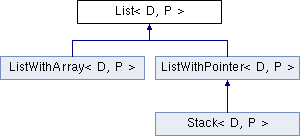
\includegraphics[height=3.000000cm]{class_list}
\end{center}
\end{figure}
\subsection*{Public Member Functions}
\begin{DoxyCompactItemize}
\item 
\hyperlink{class_list_a3deb54ab4f51c6c39aa4015f258b5812}{List} ()
\begin{DoxyCompactList}\small\item\em Constructor de la clase \hyperlink{class_list}{List}. \end{DoxyCompactList}\item 
virtual \hyperlink{class_list_a624593fb77847bf7ad4cacfba3442471}{$\sim$\+List} ()
\begin{DoxyCompactList}\small\item\em Destructor de la clase \hyperlink{class_list}{List}. \end{DoxyCompactList}\item 
virtual void \hyperlink{class_list_a01f588d87d47f8332928eca38f7b11bb}{insert} (D d)=0
\begin{DoxyCompactList}\small\item\em Metodo virtual puro para insercion de datos en \hyperlink{class_list}{List}. \end{DoxyCompactList}\item 
virtual void \hyperlink{class_list_a14fc4e853102018df78db3899aa00d71}{remove} (D d)=0
\begin{DoxyCompactList}\small\item\em Metodo virtual puro para la remocion de un dato especifico de \hyperlink{class_list}{List}. \end{DoxyCompactList}\item 
virtual P \hyperlink{class_list_a2b40d6fffc7b2fb5138b648f52c839ee}{find} (D d)=0
\begin{DoxyCompactList}\small\item\em Metodo virtual puro para la busqueda de un dato especifico en \hyperlink{class_list}{List}. \end{DoxyCompactList}\item 
virtual D \hyperlink{class_list_a5bd565e668247ae0691983227367cc88}{get} (P k)=0
\begin{DoxyCompactList}\small\item\em Metodo virtual puro para obtener un dato en \hyperlink{class_list}{List}. \end{DoxyCompactList}\item 
virtual void \hyperlink{class_list_acb062aa988f4048498b30a2d845a311b}{assign} (P k, D d)=0
\begin{DoxyCompactList}\small\item\em Metodo virtual puro para asignar un valor especifico a un dato en \hyperlink{class_list}{List}. \end{DoxyCompactList}\item 
virtual void \hyperlink{class_list_ae3795939f27cf3e688cd470450e0c27a}{sort} ()=0
\begin{DoxyCompactList}\small\item\em Metodo virtual puro para ordenar \hyperlink{class_list}{List}. \end{DoxyCompactList}\item 
virtual int \hyperlink{class_list_af213bbcf13ee436a0f04cde66e337672}{get\+Size} ()=0
\begin{DoxyCompactList}\small\item\em Metodo virtual puro para obtener el tamaño de \hyperlink{class_list}{List}. \end{DoxyCompactList}\item 
virtual void \hyperlink{class_list_a8b34931e187e7e6b86aad86510ce4f3b}{print\+List} ()=0
\begin{DoxyCompactList}\small\item\em Metodo virtual puro para imrprimir \hyperlink{class_list}{List}. \end{DoxyCompactList}\item 
virtual P \hyperlink{class_list_a4ec3e88e176bb45bc49b030d1c8abb3f}{next} (P k)=0
\begin{DoxyCompactList}\small\item\em Metodo virtual puro para obtener el siguiente elemento de una posicion especifica de \hyperlink{class_list}{List}. \end{DoxyCompactList}\item 
virtual P \hyperlink{class_list_acc1831ae92a288345ef20cb29f3846b2}{prev} (P k)=0
\begin{DoxyCompactList}\small\item\em Metodo virtual puro para obtener el elemento anterior de una posicion especifica de \hyperlink{class_list}{List}. \end{DoxyCompactList}\item 
virtual void \hyperlink{class_list_a24b4f177a70215980e81ef7b2981fa1e}{empty\+List} ()=0
\begin{DoxyCompactList}\small\item\em Metodo virtual puro para vaciar \hyperlink{class_list}{List}\+: Deja sin ningun elemento \hyperlink{class_list}{List}. \end{DoxyCompactList}\end{DoxyCompactItemize}
\subsection*{Protected Attributes}
\begin{DoxyCompactItemize}
\item 
int \hyperlink{class_list_aa61221b9bda8b2b56a61bd869daacbfd}{n}
\begin{DoxyCompactList}\small\item\em Atrib. \end{DoxyCompactList}\item 
P \hyperlink{class_list_a32b9741aa48daca064edf0e83abf7a0f}{last}
\begin{DoxyCompactList}\small\item\em Atrib. \end{DoxyCompactList}\end{DoxyCompactItemize}


\subsection{Detailed Description}
\subsubsection*{template$<$typename D, typename P$>$class List$<$ D, P $>$}

Libreria que genera un template de una clase abstracta list. 

\begin{DoxyAuthor}{Author}
Luis Adrian Aguilar -\/ B00092 

Robin Gonzalez Ricz -\/ B43011 

Giancarlo Marin -\/ B54099 
\end{DoxyAuthor}
\begin{DoxyDate}{Date}
21-\/02-\/2017 Libreria que genera un template de una clase abstracta list que toma un tipo de dato para los datos contenidos en la lista (D) y otro para los indices de las misma (P) 
\end{DoxyDate}


\subsection{Constructor \& Destructor Documentation}
\hypertarget{class_list_a3deb54ab4f51c6c39aa4015f258b5812}{\index{List@{List}!List@{List}}
\index{List@{List}!List@{List}}
\subsubsection[{List}]{\setlength{\rightskip}{0pt plus 5cm}template$<$typename D , typename P $>$ {\bf List}$<$ D, P $>$\+::{\bf List} (
\begin{DoxyParamCaption}
{}
\end{DoxyParamCaption}
)\hspace{0.3cm}{\ttfamily [inline]}}}\label{class_list_a3deb54ab4f51c6c39aa4015f258b5812}


Constructor de la clase \hyperlink{class_list}{List}. 

\hypertarget{class_list_a624593fb77847bf7ad4cacfba3442471}{\index{List@{List}!````~List@{$\sim$\+List}}
\index{````~List@{$\sim$\+List}!List@{List}}
\subsubsection[{$\sim$\+List}]{\setlength{\rightskip}{0pt plus 5cm}template$<$typename D , typename P $>$ virtual {\bf List}$<$ D, P $>$\+::$\sim${\bf List} (
\begin{DoxyParamCaption}
{}
\end{DoxyParamCaption}
)\hspace{0.3cm}{\ttfamily [inline]}, {\ttfamily [virtual]}}}\label{class_list_a624593fb77847bf7ad4cacfba3442471}


Destructor de la clase \hyperlink{class_list}{List}. 



\subsection{Member Function Documentation}
\hypertarget{class_list_acb062aa988f4048498b30a2d845a311b}{\index{List@{List}!assign@{assign}}
\index{assign@{assign}!List@{List}}
\subsubsection[{assign}]{\setlength{\rightskip}{0pt plus 5cm}template$<$typename D , typename P $>$ virtual void {\bf List}$<$ D, P $>$\+::assign (
\begin{DoxyParamCaption}
\item[{P}]{k, }
\item[{D}]{d}
\end{DoxyParamCaption}
)\hspace{0.3cm}{\ttfamily [pure virtual]}}}\label{class_list_acb062aa988f4048498b30a2d845a311b}


Metodo virtual puro para asignar un valor especifico a un dato en \hyperlink{class_list}{List}. 


\begin{DoxyParams}{Parameters}
{\em k} & Indice de tipo P dentro de list donde se asignara el nuevo valor \\
\hline
{\em d} & Dato de tipo D que se asigna en la posicion k \\
\hline
\end{DoxyParams}


Implemented in \hyperlink{class_list_with_array_a9dd1fd2337c6c8d437de71aae0e816c8}{List\+With\+Array$<$ D, P $>$}, and \hyperlink{class_list_with_pointer_aeaa834b22c4d7276a77ff29df3da7a30}{List\+With\+Pointer$<$ D, P $>$}.

\hypertarget{class_list_a24b4f177a70215980e81ef7b2981fa1e}{\index{List@{List}!empty\+List@{empty\+List}}
\index{empty\+List@{empty\+List}!List@{List}}
\subsubsection[{empty\+List}]{\setlength{\rightskip}{0pt plus 5cm}template$<$typename D , typename P $>$ virtual void {\bf List}$<$ D, P $>$\+::empty\+List (
\begin{DoxyParamCaption}
{}
\end{DoxyParamCaption}
)\hspace{0.3cm}{\ttfamily [pure virtual]}}}\label{class_list_a24b4f177a70215980e81ef7b2981fa1e}


Metodo virtual puro para vaciar \hyperlink{class_list}{List}\+: Deja sin ningun elemento \hyperlink{class_list}{List}. 



Implemented in \hyperlink{class_list_with_pointer_aec4f5374971962c79d397bbcd0080199}{List\+With\+Pointer$<$ D, P $>$}, and \hyperlink{class_list_with_array_a2179e228f285cc29b46bd5d13ba0b4ed}{List\+With\+Array$<$ D, P $>$}.

\hypertarget{class_list_a2b40d6fffc7b2fb5138b648f52c839ee}{\index{List@{List}!find@{find}}
\index{find@{find}!List@{List}}
\subsubsection[{find}]{\setlength{\rightskip}{0pt plus 5cm}template$<$typename D , typename P $>$ virtual P {\bf List}$<$ D, P $>$\+::find (
\begin{DoxyParamCaption}
\item[{D}]{d}
\end{DoxyParamCaption}
)\hspace{0.3cm}{\ttfamily [pure virtual]}}}\label{class_list_a2b40d6fffc7b2fb5138b648f52c839ee}


Metodo virtual puro para la busqueda de un dato especifico en \hyperlink{class_list}{List}. 


\begin{DoxyParams}{Parameters}
{\em d} & Dato que se desea buscar en \hyperlink{class_list}{List} \\
\hline
\end{DoxyParams}
\begin{DoxyReturn}{Returns}
Indice de tipo P dentro de \hyperlink{class_list}{List} 
\end{DoxyReturn}


Implemented in \hyperlink{class_stack_aa8a3a0b773900e44f641e3be9d9345da}{Stack$<$ D, P $>$}, \hyperlink{class_list_with_array_a9a054a6d407dc5cb39575739fe412fff}{List\+With\+Array$<$ D, P $>$}, \hyperlink{class_queue_a5c5ad7000d15506d3ec9c2ef6c8e6041}{Queue$<$ D, P $>$}, and \hyperlink{class_list_with_pointer_afeff8b963c197378553e2a3f73eaf66a}{List\+With\+Pointer$<$ D, P $>$}.

\hypertarget{class_list_a5bd565e668247ae0691983227367cc88}{\index{List@{List}!get@{get}}
\index{get@{get}!List@{List}}
\subsubsection[{get}]{\setlength{\rightskip}{0pt plus 5cm}template$<$typename D , typename P $>$ virtual D {\bf List}$<$ D, P $>$\+::get (
\begin{DoxyParamCaption}
\item[{P}]{k}
\end{DoxyParamCaption}
)\hspace{0.3cm}{\ttfamily [pure virtual]}}}\label{class_list_a5bd565e668247ae0691983227367cc88}


Metodo virtual puro para obtener un dato en \hyperlink{class_list}{List}. 


\begin{DoxyParams}{Parameters}
{\em k} & Indice de tipo P dentro de \hyperlink{class_list}{List} del que se desea obtener dato \\
\hline
\end{DoxyParams}
\begin{DoxyReturn}{Returns}
Dato contenido en k de tipo D 
\end{DoxyReturn}


Implemented in \hyperlink{class_list_with_array_a20cfc82811967bc2a77a6e43b9cebb46}{List\+With\+Array$<$ D, P $>$}, and \hyperlink{class_list_with_pointer_a0ff36c852334da8bc167356e636c1846}{List\+With\+Pointer$<$ D, P $>$}.

\hypertarget{class_list_af213bbcf13ee436a0f04cde66e337672}{\index{List@{List}!get\+Size@{get\+Size}}
\index{get\+Size@{get\+Size}!List@{List}}
\subsubsection[{get\+Size}]{\setlength{\rightskip}{0pt plus 5cm}template$<$typename D , typename P $>$ virtual int {\bf List}$<$ D, P $>$\+::get\+Size (
\begin{DoxyParamCaption}
{}
\end{DoxyParamCaption}
)\hspace{0.3cm}{\ttfamily [pure virtual]}}}\label{class_list_af213bbcf13ee436a0f04cde66e337672}


Metodo virtual puro para obtener el tamaño de \hyperlink{class_list}{List}. 



Implemented in \hyperlink{class_list_with_pointer_ac70c49b5703887fd867e90cdac3c706f}{List\+With\+Pointer$<$ D, P $>$}, \hyperlink{class_list_with_array_ae7a071bcdde9ddbf4c40a716f5a09434}{List\+With\+Array$<$ D, P $>$}, \hyperlink{class_stack_a74fc7e5921dfb247f9ad7052c3c4297a}{Stack$<$ D, P $>$}, and \hyperlink{class_queue_ab2c7217e6737bf579493b321184a2db3}{Queue$<$ D, P $>$}.

\hypertarget{class_list_a01f588d87d47f8332928eca38f7b11bb}{\index{List@{List}!insert@{insert}}
\index{insert@{insert}!List@{List}}
\subsubsection[{insert}]{\setlength{\rightskip}{0pt plus 5cm}template$<$typename D , typename P $>$ virtual void {\bf List}$<$ D, P $>$\+::insert (
\begin{DoxyParamCaption}
\item[{D}]{d}
\end{DoxyParamCaption}
)\hspace{0.3cm}{\ttfamily [pure virtual]}}}\label{class_list_a01f588d87d47f8332928eca38f7b11bb}


Metodo virtual puro para insercion de datos en \hyperlink{class_list}{List}. 


\begin{DoxyParams}{Parameters}
{\em d} & Dato de tipo D que se desea insertar en \hyperlink{class_list}{List} \\
\hline
\end{DoxyParams}


Implemented in \hyperlink{class_list_with_array_afa0b6d215c2cc1d3fe6b9b48d6b6917d}{List\+With\+Array$<$ D, P $>$}, and \hyperlink{class_list_with_pointer_a676e57683ade8e179e8eff5885f7309a}{List\+With\+Pointer$<$ D, P $>$}.

\hypertarget{class_list_a4ec3e88e176bb45bc49b030d1c8abb3f}{\index{List@{List}!next@{next}}
\index{next@{next}!List@{List}}
\subsubsection[{next}]{\setlength{\rightskip}{0pt plus 5cm}template$<$typename D , typename P $>$ virtual P {\bf List}$<$ D, P $>$\+::next (
\begin{DoxyParamCaption}
\item[{P}]{k}
\end{DoxyParamCaption}
)\hspace{0.3cm}{\ttfamily [pure virtual]}}}\label{class_list_a4ec3e88e176bb45bc49b030d1c8abb3f}


Metodo virtual puro para obtener el siguiente elemento de una posicion especifica de \hyperlink{class_list}{List}. 


\begin{DoxyParams}{Parameters}
{\em k} & Indice de tipo P dentro de \hyperlink{class_list}{List} del que se desea el siguiente elemento \\
\hline
\end{DoxyParams}
\begin{DoxyReturn}{Returns}
Siguiente elemento de k de tipo P 
\end{DoxyReturn}


Implemented in \hyperlink{class_list_with_pointer_a518b5ee89e3ad32ae7cd4ddd5d4fa7e9}{List\+With\+Pointer$<$ D, P $>$}, \hyperlink{class_list_with_array_a125811011abb77c1b11e5150f4524fb1}{List\+With\+Array$<$ D, P $>$}, \hyperlink{class_queue_aa4c9b83f260a172e1fffc389f354386f}{Queue$<$ D, P $>$}, and \hyperlink{class_stack_ab7f8f7e4ab10c00769c1debc5391fc17}{Stack$<$ D, P $>$}.

\hypertarget{class_list_acc1831ae92a288345ef20cb29f3846b2}{\index{List@{List}!prev@{prev}}
\index{prev@{prev}!List@{List}}
\subsubsection[{prev}]{\setlength{\rightskip}{0pt plus 5cm}template$<$typename D , typename P $>$ virtual P {\bf List}$<$ D, P $>$\+::prev (
\begin{DoxyParamCaption}
\item[{P}]{k}
\end{DoxyParamCaption}
)\hspace{0.3cm}{\ttfamily [pure virtual]}}}\label{class_list_acc1831ae92a288345ef20cb29f3846b2}


Metodo virtual puro para obtener el elemento anterior de una posicion especifica de \hyperlink{class_list}{List}. 


\begin{DoxyParams}{Parameters}
{\em k} & Indice de tipo P dentro de \hyperlink{class_list}{List} del que se desea el elemento anterior \\
\hline
\end{DoxyParams}
\begin{DoxyReturn}{Returns}
Elemento anterior de k de tipo P 
\end{DoxyReturn}


Implemented in \hyperlink{class_list_with_pointer_a7242068fcc3a193f0f7e94517856e431}{List\+With\+Pointer$<$ D, P $>$}, \hyperlink{class_list_with_array_a72f0d74c4ae1fd4697088114db41d442}{List\+With\+Array$<$ D, P $>$}, \hyperlink{class_queue_adcb9a0e709ea65bc7e98f7e9cbae8a39}{Queue$<$ D, P $>$}, and \hyperlink{class_stack_a0c0b55f72c9249bfb9252bce1a93458d}{Stack$<$ D, P $>$}.

\hypertarget{class_list_a8b34931e187e7e6b86aad86510ce4f3b}{\index{List@{List}!print\+List@{print\+List}}
\index{print\+List@{print\+List}!List@{List}}
\subsubsection[{print\+List}]{\setlength{\rightskip}{0pt plus 5cm}template$<$typename D , typename P $>$ virtual void {\bf List}$<$ D, P $>$\+::print\+List (
\begin{DoxyParamCaption}
{}
\end{DoxyParamCaption}
)\hspace{0.3cm}{\ttfamily [pure virtual]}}}\label{class_list_a8b34931e187e7e6b86aad86510ce4f3b}


Metodo virtual puro para imrprimir \hyperlink{class_list}{List}. 



Implemented in \hyperlink{class_list_with_pointer_a7079b5f1dbddb87a7e33ffc71ebb7b92}{List\+With\+Pointer$<$ D, P $>$}, and \hyperlink{class_list_with_array_a515ea38cb40ba7b0c9df98825b2dd270}{List\+With\+Array$<$ D, P $>$}.

\hypertarget{class_list_a14fc4e853102018df78db3899aa00d71}{\index{List@{List}!remove@{remove}}
\index{remove@{remove}!List@{List}}
\subsubsection[{remove}]{\setlength{\rightskip}{0pt plus 5cm}template$<$typename D , typename P $>$ virtual void {\bf List}$<$ D, P $>$\+::remove (
\begin{DoxyParamCaption}
\item[{D}]{d}
\end{DoxyParamCaption}
)\hspace{0.3cm}{\ttfamily [pure virtual]}}}\label{class_list_a14fc4e853102018df78db3899aa00d71}


Metodo virtual puro para la remocion de un dato especifico de \hyperlink{class_list}{List}. 


\begin{DoxyParams}{Parameters}
{\em d} & Dato de tipo D que se desea remover de \hyperlink{class_list}{List} \\
\hline
\end{DoxyParams}


Implemented in \hyperlink{class_list_with_array_aaa18e76fc128ca05151178d914901ec3}{List\+With\+Array$<$ D, P $>$}, and \hyperlink{class_list_with_pointer_abcb151e95e9fffea7f9f7af593d8176f}{List\+With\+Pointer$<$ D, P $>$}.

\hypertarget{class_list_ae3795939f27cf3e688cd470450e0c27a}{\index{List@{List}!sort@{sort}}
\index{sort@{sort}!List@{List}}
\subsubsection[{sort}]{\setlength{\rightskip}{0pt plus 5cm}template$<$typename D , typename P $>$ virtual void {\bf List}$<$ D, P $>$\+::sort (
\begin{DoxyParamCaption}
{}
\end{DoxyParamCaption}
)\hspace{0.3cm}{\ttfamily [pure virtual]}}}\label{class_list_ae3795939f27cf3e688cd470450e0c27a}


Metodo virtual puro para ordenar \hyperlink{class_list}{List}. 



Implemented in \hyperlink{class_list_with_array_a1a0ec4ab4a8fcb1a20568445ad892c9a}{List\+With\+Array$<$ D, P $>$}, \hyperlink{class_list_with_pointer_aa46631b2da29895d1f767626fb591bc8}{List\+With\+Pointer$<$ D, P $>$}, and \hyperlink{class_queue_a896b0e1bcac0d660079eb838c1823446}{Queue$<$ D, P $>$}.



\subsection{Member Data Documentation}
\hypertarget{class_list_a32b9741aa48daca064edf0e83abf7a0f}{\index{List@{List}!last@{last}}
\index{last@{last}!List@{List}}
\subsubsection[{last}]{\setlength{\rightskip}{0pt plus 5cm}template$<$typename D , typename P $>$ P {\bf List}$<$ D, P $>$\+::last\hspace{0.3cm}{\ttfamily [protected]}}}\label{class_list_a32b9741aa48daca064edf0e83abf7a0f}


Atrib. 

protegido de tipo P que indica el indice del ultimo elemento de list \hypertarget{class_list_aa61221b9bda8b2b56a61bd869daacbfd}{\index{List@{List}!n@{n}}
\index{n@{n}!List@{List}}
\subsubsection[{n}]{\setlength{\rightskip}{0pt plus 5cm}template$<$typename D , typename P $>$ int {\bf List}$<$ D, P $>$\+::n\hspace{0.3cm}{\ttfamily [protected]}}}\label{class_list_aa61221b9bda8b2b56a61bd869daacbfd}


Atrib. 

protegido de tipo entero que indica el numero de elementos en list 

The documentation for this class was generated from the following file\+:\begin{DoxyCompactItemize}
\item 
include/\hyperlink{_list_8h}{List.\+h}\end{DoxyCompactItemize}

\hypertarget{class_list_with_array}{\section{List\+With\+Array$<$ D, P $>$ Class Template Reference}
\label{class_list_with_array}\index{List\+With\+Array$<$ D, P $>$@{List\+With\+Array$<$ D, P $>$}}
}


Libreria que genera un template de una clase \hyperlink{class_list_with_array}{List\+With\+Array} (lista implementada con arreglos) que hereda de la clase \hyperlink{class_list}{List} y que toma un tipo de dato para los datos contenidos en la lista (D) y otro para los indices de las misma (P)  




{\ttfamily \#include $<$List\+With\+Array.\+h$>$}



Inheritance diagram for List\+With\+Array$<$ D, P $>$\+:


Collaboration diagram for List\+With\+Array$<$ D, P $>$\+:
\subsection*{Public Member Functions}
\begin{DoxyCompactItemize}
\item 
\hyperlink{class_list_with_array_a06f0e8035e9cc43aff4d32c46a00fcf0}{List\+With\+Array} ()
\begin{DoxyCompactList}\small\item\em Constructor de la clase \hyperlink{class_list_with_array}{List\+With\+Array}. \end{DoxyCompactList}\item 
\hyperlink{class_list_with_array_a3a6d11f203fb0f7e458672e85db26b03}{List\+With\+Array} (int t)
\begin{DoxyCompactList}\small\item\em Constructor sobrecargado de la clase \hyperlink{class_list_with_array}{List\+With\+Array}. \end{DoxyCompactList}\item 
\hyperlink{class_list_with_array_a1886482555430b0f3eb5ebe02cbb0c87}{$\sim$\+List\+With\+Array} ()
\begin{DoxyCompactList}\small\item\em Destructor de la clase \hyperlink{class_list_with_array}{List\+With\+Array}. \end{DoxyCompactList}\item 
void \hyperlink{class_list_with_array_afa0b6d215c2cc1d3fe6b9b48d6b6917d}{insert} (\hyperlink{main_8cpp_af316c33cc298530f245e8b55330e86b5}{D} d)
\begin{DoxyCompactList}\small\item\em Metodo que implementa la insercion para \hyperlink{class_list_with_array}{List\+With\+Array}. \end{DoxyCompactList}\item 
void \hyperlink{class_list_with_array_aaa18e76fc128ca05151178d914901ec3}{remove} (\hyperlink{main_8cpp_af316c33cc298530f245e8b55330e86b5}{D} d)
\begin{DoxyCompactList}\small\item\em Metodo que implementa la remocion para \hyperlink{class_list_with_array}{List\+With\+Array}. \end{DoxyCompactList}\item 
P \hyperlink{class_list_with_array_a9a054a6d407dc5cb39575739fe412fff}{find} (\hyperlink{main_8cpp_af316c33cc298530f245e8b55330e86b5}{D} d)
\begin{DoxyCompactList}\small\item\em Metodo que implementa la busqueda para \hyperlink{class_list_with_array}{List\+With\+Array}. \end{DoxyCompactList}\item 
\hyperlink{main_8cpp_af316c33cc298530f245e8b55330e86b5}{D} \hyperlink{class_list_with_array_a20cfc82811967bc2a77a6e43b9cebb46}{get} (P k)
\begin{DoxyCompactList}\small\item\em Metodo que implementa el obtener un dato para \hyperlink{class_list_with_array}{List\+With\+Array}. \end{DoxyCompactList}\item 
void \hyperlink{class_list_with_array_a9dd1fd2337c6c8d437de71aae0e816c8}{assign} (P k, \hyperlink{main_8cpp_af316c33cc298530f245e8b55330e86b5}{D} d)
\begin{DoxyCompactList}\small\item\em Metodo que implementa el asignar un valor especifico a un dato en \hyperlink{class_list_with_array}{List\+With\+Array}. \end{DoxyCompactList}\item 
void \hyperlink{class_list_with_array_a1a0ec4ab4a8fcb1a20568445ad892c9a}{sort} ()
\begin{DoxyCompactList}\small\item\em Metodo que implementa el ordenar para \hyperlink{class_list_with_array}{List\+With\+Array}. \end{DoxyCompactList}\item 
int \hyperlink{class_list_with_array_ae7a071bcdde9ddbf4c40a716f5a09434}{get\+Size} ()
\begin{DoxyCompactList}\small\item\em Metodo que implementa el obtener tamaño de \hyperlink{class_list_with_array}{List\+With\+Array}. \end{DoxyCompactList}\item 
void \hyperlink{class_list_with_array_a515ea38cb40ba7b0c9df98825b2dd270}{print\+List} ()
\begin{DoxyCompactList}\small\item\em Metodo que implementa el imrprimir lista para \hyperlink{class_list_with_array}{List\+With\+Array}. \end{DoxyCompactList}\item 
P \hyperlink{class_list_with_array_a125811011abb77c1b11e5150f4524fb1}{next} (P k)
\begin{DoxyCompactList}\small\item\em Metodo que implementa el obtener siguiente elemento de una posicion especifica de \hyperlink{class_list_with_array}{List\+With\+Array}. \end{DoxyCompactList}\item 
P \hyperlink{class_list_with_array_a72f0d74c4ae1fd4697088114db41d442}{prev} (P k)
\begin{DoxyCompactList}\small\item\em Metodo que implementa el obtener elemento anterior de una posicion especifica de \hyperlink{class_list_with_array}{List\+With\+Array}. \end{DoxyCompactList}\item 
void \hyperlink{class_list_with_array_a2179e228f285cc29b46bd5d13ba0b4ed}{empty\+List} ()
\begin{DoxyCompactList}\small\item\em Metodo que implementa el vaciar Lista que Deja sin ningun elemento a \hyperlink{class_list_with_array}{List\+With\+Array}. \end{DoxyCompactList}\end{DoxyCompactItemize}
\subsection*{Additional Inherited Members}


\subsection{Detailed Description}
\subsubsection*{template$<$typename D, typename P$>$class List\+With\+Array$<$ D, P $>$}

Libreria que genera un template de una clase \hyperlink{class_list_with_array}{List\+With\+Array} (lista implementada con arreglos) que hereda de la clase \hyperlink{class_list}{List} y que toma un tipo de dato para los datos contenidos en la lista (D) y otro para los indices de las misma (P) 

Definition at line 16 of file List\+With\+Array.\+h.



\subsection{Constructor \& Destructor Documentation}
\hypertarget{class_list_with_array_a06f0e8035e9cc43aff4d32c46a00fcf0}{\index{List\+With\+Array@{List\+With\+Array}!List\+With\+Array@{List\+With\+Array}}
\index{List\+With\+Array@{List\+With\+Array}!List\+With\+Array@{List\+With\+Array}}
\subsubsection[{List\+With\+Array}]{\setlength{\rightskip}{0pt plus 5cm}template$<$typename D, typename P$>$ {\bf List\+With\+Array}$<$ {\bf D}, P $>$\+::{\bf List\+With\+Array} (
\begin{DoxyParamCaption}
{}
\end{DoxyParamCaption}
)\hspace{0.3cm}{\ttfamily [inline]}}}\label{class_list_with_array_a06f0e8035e9cc43aff4d32c46a00fcf0}


Constructor de la clase \hyperlink{class_list_with_array}{List\+With\+Array}. 



Definition at line 22 of file List\+With\+Array.\+h.

\hypertarget{class_list_with_array_a3a6d11f203fb0f7e458672e85db26b03}{\index{List\+With\+Array@{List\+With\+Array}!List\+With\+Array@{List\+With\+Array}}
\index{List\+With\+Array@{List\+With\+Array}!List\+With\+Array@{List\+With\+Array}}
\subsubsection[{List\+With\+Array}]{\setlength{\rightskip}{0pt plus 5cm}template$<$typename D, typename P$>$ {\bf List\+With\+Array}$<$ {\bf D}, P $>$\+::{\bf List\+With\+Array} (
\begin{DoxyParamCaption}
\item[{int}]{t}
\end{DoxyParamCaption}
)\hspace{0.3cm}{\ttfamily [inline]}}}\label{class_list_with_array_a3a6d11f203fb0f7e458672e85db26b03}


Constructor sobrecargado de la clase \hyperlink{class_list_with_array}{List\+With\+Array}. 


\begin{DoxyParams}{Parameters}
{\em t} & Entero que determina la cantidad maxima de elementon que puede contener la lista \\
\hline
\end{DoxyParams}


Definition at line 32 of file List\+With\+Array.\+h.

\hypertarget{class_list_with_array_a1886482555430b0f3eb5ebe02cbb0c87}{\index{List\+With\+Array@{List\+With\+Array}!````~List\+With\+Array@{$\sim$\+List\+With\+Array}}
\index{````~List\+With\+Array@{$\sim$\+List\+With\+Array}!List\+With\+Array@{List\+With\+Array}}
\subsubsection[{$\sim$\+List\+With\+Array}]{\setlength{\rightskip}{0pt plus 5cm}template$<$typename D, typename P$>$ {\bf List\+With\+Array}$<$ {\bf D}, P $>$\+::$\sim${\bf List\+With\+Array} (
\begin{DoxyParamCaption}
{}
\end{DoxyParamCaption}
)\hspace{0.3cm}{\ttfamily [inline]}}}\label{class_list_with_array_a1886482555430b0f3eb5ebe02cbb0c87}


Destructor de la clase \hyperlink{class_list_with_array}{List\+With\+Array}. 



Definition at line 41 of file List\+With\+Array.\+h.



\subsection{Member Function Documentation}
\hypertarget{class_list_with_array_a9dd1fd2337c6c8d437de71aae0e816c8}{\index{List\+With\+Array@{List\+With\+Array}!assign@{assign}}
\index{assign@{assign}!List\+With\+Array@{List\+With\+Array}}
\subsubsection[{assign}]{\setlength{\rightskip}{0pt plus 5cm}template$<$typename D, typename P$>$ void {\bf List\+With\+Array}$<$ {\bf D}, P $>$\+::assign (
\begin{DoxyParamCaption}
\item[{P}]{k, }
\item[{{\bf D}}]{d}
\end{DoxyParamCaption}
)\hspace{0.3cm}{\ttfamily [inline]}, {\ttfamily [virtual]}}}\label{class_list_with_array_a9dd1fd2337c6c8d437de71aae0e816c8}


Metodo que implementa el asignar un valor especifico a un dato en \hyperlink{class_list_with_array}{List\+With\+Array}. 


\begin{DoxyParams}{Parameters}
{\em k} & Indice de tipo P dentro de list donde se asignara el nuevo valor \\
\hline
{\em d} & Dato de tipo D que se asigna en la posicion k \\
\hline
\end{DoxyParams}


Implements \hyperlink{class_list_acb062aa988f4048498b30a2d845a311b}{List$<$ D, P $>$}.



Definition at line 122 of file List\+With\+Array.\+h.

\hypertarget{class_list_with_array_a2179e228f285cc29b46bd5d13ba0b4ed}{\index{List\+With\+Array@{List\+With\+Array}!empty\+List@{empty\+List}}
\index{empty\+List@{empty\+List}!List\+With\+Array@{List\+With\+Array}}
\subsubsection[{empty\+List}]{\setlength{\rightskip}{0pt plus 5cm}template$<$typename D, typename P$>$ void {\bf List\+With\+Array}$<$ {\bf D}, P $>$\+::empty\+List (
\begin{DoxyParamCaption}
{}
\end{DoxyParamCaption}
)\hspace{0.3cm}{\ttfamily [inline]}, {\ttfamily [virtual]}}}\label{class_list_with_array_a2179e228f285cc29b46bd5d13ba0b4ed}


Metodo que implementa el vaciar Lista que Deja sin ningun elemento a \hyperlink{class_list_with_array}{List\+With\+Array}. 



Implements \hyperlink{class_list_a24b4f177a70215980e81ef7b2981fa1e}{List$<$ D, P $>$}.



Definition at line 190 of file List\+With\+Array.\+h.

\hypertarget{class_list_with_array_a9a054a6d407dc5cb39575739fe412fff}{\index{List\+With\+Array@{List\+With\+Array}!find@{find}}
\index{find@{find}!List\+With\+Array@{List\+With\+Array}}
\subsubsection[{find}]{\setlength{\rightskip}{0pt plus 5cm}template$<$typename D, typename P$>$ P {\bf List\+With\+Array}$<$ {\bf D}, P $>$\+::find (
\begin{DoxyParamCaption}
\item[{{\bf D}}]{d}
\end{DoxyParamCaption}
)\hspace{0.3cm}{\ttfamily [inline]}, {\ttfamily [virtual]}}}\label{class_list_with_array_a9a054a6d407dc5cb39575739fe412fff}


Metodo que implementa la busqueda para \hyperlink{class_list_with_array}{List\+With\+Array}. 


\begin{DoxyParams}{Parameters}
{\em d} & Dato que se desea buscar en \hyperlink{class_list}{List} \\
\hline
\end{DoxyParams}
\begin{DoxyReturn}{Returns}
Indice de tipo P dentro de \hyperlink{class_list}{List} 
\end{DoxyReturn}
Indicacion de que el dato no fue encontrado en la lista 

Implements \hyperlink{class_list_a2b40d6fffc7b2fb5138b648f52c839ee}{List$<$ D, P $>$}.



Definition at line 100 of file List\+With\+Array.\+h.

\hypertarget{class_list_with_array_a20cfc82811967bc2a77a6e43b9cebb46}{\index{List\+With\+Array@{List\+With\+Array}!get@{get}}
\index{get@{get}!List\+With\+Array@{List\+With\+Array}}
\subsubsection[{get}]{\setlength{\rightskip}{0pt plus 5cm}template$<$typename D, typename P$>$ {\bf D} {\bf List\+With\+Array}$<$ {\bf D}, P $>$\+::get (
\begin{DoxyParamCaption}
\item[{P}]{k}
\end{DoxyParamCaption}
)\hspace{0.3cm}{\ttfamily [inline]}, {\ttfamily [virtual]}}}\label{class_list_with_array_a20cfc82811967bc2a77a6e43b9cebb46}


Metodo que implementa el obtener un dato para \hyperlink{class_list_with_array}{List\+With\+Array}. 


\begin{DoxyParams}{Parameters}
{\em k} & Indice de tipo P dentro de \hyperlink{class_list}{List} del que se desea obtener dato \\
\hline
\end{DoxyParams}
\begin{DoxyReturn}{Returns}
Dato contenido en k de tipo D 
\end{DoxyReturn}


Implements \hyperlink{class_list_a5bd565e668247ae0691983227367cc88}{List$<$ D, P $>$}.



Definition at line 113 of file List\+With\+Array.\+h.

\hypertarget{class_list_with_array_ae7a071bcdde9ddbf4c40a716f5a09434}{\index{List\+With\+Array@{List\+With\+Array}!get\+Size@{get\+Size}}
\index{get\+Size@{get\+Size}!List\+With\+Array@{List\+With\+Array}}
\subsubsection[{get\+Size}]{\setlength{\rightskip}{0pt plus 5cm}template$<$typename D, typename P$>$ int {\bf List\+With\+Array}$<$ {\bf D}, P $>$\+::get\+Size (
\begin{DoxyParamCaption}
{}
\end{DoxyParamCaption}
)\hspace{0.3cm}{\ttfamily [inline]}, {\ttfamily [virtual]}}}\label{class_list_with_array_ae7a071bcdde9ddbf4c40a716f5a09434}


Metodo que implementa el obtener tamaño de \hyperlink{class_list_with_array}{List\+With\+Array}. 



Implements \hyperlink{class_list_af213bbcf13ee436a0f04cde66e337672}{List$<$ D, P $>$}.



Definition at line 149 of file List\+With\+Array.\+h.

\hypertarget{class_list_with_array_afa0b6d215c2cc1d3fe6b9b48d6b6917d}{\index{List\+With\+Array@{List\+With\+Array}!insert@{insert}}
\index{insert@{insert}!List\+With\+Array@{List\+With\+Array}}
\subsubsection[{insert}]{\setlength{\rightskip}{0pt plus 5cm}template$<$typename D, typename P$>$ void {\bf List\+With\+Array}$<$ {\bf D}, P $>$\+::insert (
\begin{DoxyParamCaption}
\item[{{\bf D}}]{d}
\end{DoxyParamCaption}
)\hspace{0.3cm}{\ttfamily [inline]}, {\ttfamily [virtual]}}}\label{class_list_with_array_afa0b6d215c2cc1d3fe6b9b48d6b6917d}


Metodo que implementa la insercion para \hyperlink{class_list_with_array}{List\+With\+Array}. 


\begin{DoxyParams}{Parameters}
{\em d} & Dato de tipo D que se desea insertar en \hyperlink{class_list}{List} \\
\hline
\end{DoxyParams}


Implements \hyperlink{class_list_a01f588d87d47f8332928eca38f7b11bb}{List$<$ D, P $>$}.



Definition at line 50 of file List\+With\+Array.\+h.

\hypertarget{class_list_with_array_a125811011abb77c1b11e5150f4524fb1}{\index{List\+With\+Array@{List\+With\+Array}!next@{next}}
\index{next@{next}!List\+With\+Array@{List\+With\+Array}}
\subsubsection[{next}]{\setlength{\rightskip}{0pt plus 5cm}template$<$typename D, typename P$>$ P {\bf List\+With\+Array}$<$ {\bf D}, P $>$\+::next (
\begin{DoxyParamCaption}
\item[{P}]{k}
\end{DoxyParamCaption}
)\hspace{0.3cm}{\ttfamily [inline]}, {\ttfamily [virtual]}}}\label{class_list_with_array_a125811011abb77c1b11e5150f4524fb1}


Metodo que implementa el obtener siguiente elemento de una posicion especifica de \hyperlink{class_list_with_array}{List\+With\+Array}. 


\begin{DoxyParams}{Parameters}
{\em k} & Indice de tipo P dentro de \hyperlink{class_list}{List} del que se desea el siguiente elemento \\
\hline
\end{DoxyParams}
\begin{DoxyReturn}{Returns}
Siguiente elemento de k de tipo P 
\end{DoxyReturn}
Indicacion de que no hay dato siguiente en la lista 

Implements \hyperlink{class_list_a4ec3e88e176bb45bc49b030d1c8abb3f}{List$<$ D, P $>$}.



Definition at line 168 of file List\+With\+Array.\+h.

\hypertarget{class_list_with_array_a72f0d74c4ae1fd4697088114db41d442}{\index{List\+With\+Array@{List\+With\+Array}!prev@{prev}}
\index{prev@{prev}!List\+With\+Array@{List\+With\+Array}}
\subsubsection[{prev}]{\setlength{\rightskip}{0pt plus 5cm}template$<$typename D, typename P$>$ P {\bf List\+With\+Array}$<$ {\bf D}, P $>$\+::prev (
\begin{DoxyParamCaption}
\item[{P}]{k}
\end{DoxyParamCaption}
)\hspace{0.3cm}{\ttfamily [inline]}, {\ttfamily [virtual]}}}\label{class_list_with_array_a72f0d74c4ae1fd4697088114db41d442}


Metodo que implementa el obtener elemento anterior de una posicion especifica de \hyperlink{class_list_with_array}{List\+With\+Array}. 


\begin{DoxyParams}{Parameters}
{\em k} & Indice de tipo P dentro de \hyperlink{class_list}{List} del que se desea el elemento anterior \\
\hline
\end{DoxyParams}
\begin{DoxyReturn}{Returns}
Elemento anterior de k de tipo P 
\end{DoxyReturn}
Indicacion de que no hay dato anterior en la lista 

Implements \hyperlink{class_list_acc1831ae92a288345ef20cb29f3846b2}{List$<$ D, P $>$}.



Definition at line 180 of file List\+With\+Array.\+h.

\hypertarget{class_list_with_array_a515ea38cb40ba7b0c9df98825b2dd270}{\index{List\+With\+Array@{List\+With\+Array}!print\+List@{print\+List}}
\index{print\+List@{print\+List}!List\+With\+Array@{List\+With\+Array}}
\subsubsection[{print\+List}]{\setlength{\rightskip}{0pt plus 5cm}template$<$typename D, typename P$>$ void {\bf List\+With\+Array}$<$ {\bf D}, P $>$\+::print\+List (
\begin{DoxyParamCaption}
{}
\end{DoxyParamCaption}
)\hspace{0.3cm}{\ttfamily [inline]}, {\ttfamily [virtual]}}}\label{class_list_with_array_a515ea38cb40ba7b0c9df98825b2dd270}


Metodo que implementa el imrprimir lista para \hyperlink{class_list_with_array}{List\+With\+Array}. 



Implements \hyperlink{class_list_a8b34931e187e7e6b86aad86510ce4f3b}{List$<$ D, P $>$}.



Definition at line 156 of file List\+With\+Array.\+h.

\hypertarget{class_list_with_array_aaa18e76fc128ca05151178d914901ec3}{\index{List\+With\+Array@{List\+With\+Array}!remove@{remove}}
\index{remove@{remove}!List\+With\+Array@{List\+With\+Array}}
\subsubsection[{remove}]{\setlength{\rightskip}{0pt plus 5cm}template$<$typename D, typename P$>$ void {\bf List\+With\+Array}$<$ {\bf D}, P $>$\+::remove (
\begin{DoxyParamCaption}
\item[{{\bf D}}]{d}
\end{DoxyParamCaption}
)\hspace{0.3cm}{\ttfamily [inline]}, {\ttfamily [virtual]}}}\label{class_list_with_array_aaa18e76fc128ca05151178d914901ec3}


Metodo que implementa la remocion para \hyperlink{class_list_with_array}{List\+With\+Array}. 


\begin{DoxyParams}{Parameters}
{\em d} & Dato de tipo D que se desea remover de \hyperlink{class_list}{List} \\
\hline
\end{DoxyParams}
$<$entero que indica la posicion donde se debe remover 

Implements \hyperlink{class_list_a14fc4e853102018df78db3899aa00d71}{List$<$ D, P $>$}.



Definition at line 84 of file List\+With\+Array.\+h.

\hypertarget{class_list_with_array_a1a0ec4ab4a8fcb1a20568445ad892c9a}{\index{List\+With\+Array@{List\+With\+Array}!sort@{sort}}
\index{sort@{sort}!List\+With\+Array@{List\+With\+Array}}
\subsubsection[{sort}]{\setlength{\rightskip}{0pt plus 5cm}template$<$typename D, typename P$>$ void {\bf List\+With\+Array}$<$ {\bf D}, P $>$\+::sort (
\begin{DoxyParamCaption}
{}
\end{DoxyParamCaption}
)\hspace{0.3cm}{\ttfamily [inline]}, {\ttfamily [virtual]}}}\label{class_list_with_array_a1a0ec4ab4a8fcb1a20568445ad892c9a}


Metodo que implementa el ordenar para \hyperlink{class_list_with_array}{List\+With\+Array}. 

Implementacion por medio de Selection Sort 

Implements \hyperlink{class_list_ae3795939f27cf3e688cd470450e0c27a}{List$<$ D, P $>$}.



Definition at line 129 of file List\+With\+Array.\+h.



The documentation for this class was generated from the following file\+:\begin{DoxyCompactItemize}
\item 
include/\hyperlink{_list_with_array_8h}{List\+With\+Array.\+h}\end{DoxyCompactItemize}

\hypertarget{class_stade}{\section{Stade Class Reference}
\label{class_stade}\index{Stade@{Stade}}
}


{\ttfamily \#include $<$Stade.\+h$>$}

\subsection*{Public Member Functions}
\begin{DoxyCompactItemize}
\item 
\hyperlink{class_stade_a0b456ba62c0e36e23770d7f97bb090e7}{Stade} ()
\begin{DoxyCompactList}\small\item\em Constructor de la clase \hyperlink{class_stade}{Stade}. \end{DoxyCompactList}\item 
\hyperlink{class_stade_a7bdc8d5eb5e36b31e4ad46e58447cd48}{Stade} (int $\ast$t)
\begin{DoxyCompactList}\small\item\em Constructor sobrecargado de la clase Data. \end{DoxyCompactList}\item 
\hyperlink{class_stade_abdea3c92c222929ebf3c6f5615085529}{$\sim$\+Stade} ()
\begin{DoxyCompactList}\small\item\em Destructor de la clase \hyperlink{class_stade}{Stade}. \end{DoxyCompactList}\end{DoxyCompactItemize}
\subsection*{Public Attributes}
\begin{DoxyCompactItemize}
\item 
int $\ast$ \hyperlink{class_stade_ad941a9ee2d5283e933be7dc4bb6096fc}{tag}
\item 
bool \hyperlink{class_stade_a4f818739089a18e7bba2f8187088fb9b}{success100}
\begin{DoxyCompactList}\small\item\em Atrib. publico de tipo int que contiene el tag del estado///. \end{DoxyCompactList}\item 
bool \hyperlink{class_stade_a108a9c100d92ca8a822516376c79ac77}{success\+Les100}
\begin{DoxyCompactList}\small\item\em Atrib. publico que indica si es un caso de exito del 100\%///. \end{DoxyCompactList}\end{DoxyCompactItemize}


\subsection{Detailed Description}


Definition at line 12 of file Stade.\+h.



\subsection{Constructor \& Destructor Documentation}
\hypertarget{class_stade_a0b456ba62c0e36e23770d7f97bb090e7}{\index{Stade@{Stade}!Stade@{Stade}}
\index{Stade@{Stade}!Stade@{Stade}}
\subsubsection[{Stade}]{\setlength{\rightskip}{0pt plus 5cm}Stade\+::\+Stade (
\begin{DoxyParamCaption}
{}
\end{DoxyParamCaption}
)\hspace{0.3cm}{\ttfamily [inline]}}}\label{class_stade_a0b456ba62c0e36e23770d7f97bb090e7}


Constructor de la clase \hyperlink{class_stade}{Stade}. 



Definition at line 21 of file Stade.\+h.

\hypertarget{class_stade_a7bdc8d5eb5e36b31e4ad46e58447cd48}{\index{Stade@{Stade}!Stade@{Stade}}
\index{Stade@{Stade}!Stade@{Stade}}
\subsubsection[{Stade}]{\setlength{\rightskip}{0pt plus 5cm}Stade\+::\+Stade (
\begin{DoxyParamCaption}
\item[{int $\ast$}]{t}
\end{DoxyParamCaption}
)\hspace{0.3cm}{\ttfamily [inline]}}}\label{class_stade_a7bdc8d5eb5e36b31e4ad46e58447cd48}


Constructor sobrecargado de la clase Data. 


\begin{DoxyParams}{Parameters}
{\em d} & Tipo int con el tag a guardar \\
\hline
\end{DoxyParams}


Definition at line 31 of file Stade.\+h.

\hypertarget{class_stade_abdea3c92c222929ebf3c6f5615085529}{\index{Stade@{Stade}!````~Stade@{$\sim$\+Stade}}
\index{````~Stade@{$\sim$\+Stade}!Stade@{Stade}}
\subsubsection[{$\sim$\+Stade}]{\setlength{\rightskip}{0pt plus 5cm}Stade\+::$\sim$\+Stade (
\begin{DoxyParamCaption}
{}
\end{DoxyParamCaption}
)\hspace{0.3cm}{\ttfamily [inline]}}}\label{class_stade_abdea3c92c222929ebf3c6f5615085529}


Destructor de la clase \hyperlink{class_stade}{Stade}. 



Definition at line 40 of file Stade.\+h.



\subsection{Member Data Documentation}
\hypertarget{class_stade_a4f818739089a18e7bba2f8187088fb9b}{\index{Stade@{Stade}!success100@{success100}}
\index{success100@{success100}!Stade@{Stade}}
\subsubsection[{success100}]{\setlength{\rightskip}{0pt plus 5cm}bool Stade\+::success100}}\label{class_stade_a4f818739089a18e7bba2f8187088fb9b}


Atrib. publico de tipo int que contiene el tag del estado///. 



Definition at line 15 of file Stade.\+h.

\hypertarget{class_stade_a108a9c100d92ca8a822516376c79ac77}{\index{Stade@{Stade}!success\+Les100@{success\+Les100}}
\index{success\+Les100@{success\+Les100}!Stade@{Stade}}
\subsubsection[{success\+Les100}]{\setlength{\rightskip}{0pt plus 5cm}bool Stade\+::success\+Les100}}\label{class_stade_a108a9c100d92ca8a822516376c79ac77}


Atrib. publico que indica si es un caso de exito del 100\%///. 



Definition at line 16 of file Stade.\+h.

\hypertarget{class_stade_ad941a9ee2d5283e933be7dc4bb6096fc}{\index{Stade@{Stade}!tag@{tag}}
\index{tag@{tag}!Stade@{Stade}}
\subsubsection[{tag}]{\setlength{\rightskip}{0pt plus 5cm}int$\ast$ Stade\+::tag}}\label{class_stade_ad941a9ee2d5283e933be7dc4bb6096fc}


Definition at line 14 of file Stade.\+h.



The documentation for this class was generated from the following file\+:\begin{DoxyCompactItemize}
\item 
include/\hyperlink{_stade_8h}{Stade.\+h}\end{DoxyCompactItemize}

\hypertarget{class_stade_suc}{\section{Stade\+Suc Class Reference}
\label{class_stade_suc}\index{Stade\+Suc@{Stade\+Suc}}
}


{\ttfamily \#include $<$Stade\+Suc.\+h$>$}

\subsection*{Public Member Functions}
\begin{DoxyCompactItemize}
\item 
\hyperlink{class_stade_suc_ae069c77a99d27cf9f3bd37253b19c146}{Stade\+Suc} ()
\begin{DoxyCompactList}\small\item\em Atrib. publico de tipo int que indica el numero de palabra que corresponde el estado de exito///. \end{DoxyCompactList}\item 
\hyperlink{class_stade_suc_aee378a96e88aceea354d7a946d1d535e}{Stade\+Suc} (int i, int n)
\begin{DoxyCompactList}\small\item\em Constructor sobrecargado de la clase \hyperlink{class_stade_suc}{Stade\+Suc}. \end{DoxyCompactList}\item 
\hyperlink{class_stade_suc_acf19e9a05be93424f68acff2deafad4a}{$\sim$\+Stade\+Suc} ()
\begin{DoxyCompactList}\small\item\em Destructor de la clase \hyperlink{class_stade}{Stade}. \end{DoxyCompactList}\end{DoxyCompactItemize}
\subsection*{Public Attributes}
\begin{DoxyCompactItemize}
\item 
int \hyperlink{class_stade_suc_a32866d1f7785fc1a3208a161346ba85f}{index}
\item 
int \hyperlink{class_stade_suc_a9fd058e20b7c620287c5fde47f2d2839}{num\+Word}
\begin{DoxyCompactList}\small\item\em Atrib. publico de tipo int que indica el indice donde sucedio el exito///. \end{DoxyCompactList}\end{DoxyCompactItemize}


\subsection{Detailed Description}


Definition at line 12 of file Stade\+Suc.\+h.



\subsection{Constructor \& Destructor Documentation}
\hypertarget{class_stade_suc_ae069c77a99d27cf9f3bd37253b19c146}{\index{Stade\+Suc@{Stade\+Suc}!Stade\+Suc@{Stade\+Suc}}
\index{Stade\+Suc@{Stade\+Suc}!Stade\+Suc@{Stade\+Suc}}
\subsubsection[{Stade\+Suc}]{\setlength{\rightskip}{0pt plus 5cm}Stade\+Suc\+::\+Stade\+Suc (
\begin{DoxyParamCaption}
{}
\end{DoxyParamCaption}
)\hspace{0.3cm}{\ttfamily [inline]}}}\label{class_stade_suc_ae069c77a99d27cf9f3bd37253b19c146}


Atrib. publico de tipo int que indica el numero de palabra que corresponde el estado de exito///. 

Constructor de la clase \hyperlink{class_stade_suc}{Stade\+Suc} 

Definition at line 20 of file Stade\+Suc.\+h.

\hypertarget{class_stade_suc_aee378a96e88aceea354d7a946d1d535e}{\index{Stade\+Suc@{Stade\+Suc}!Stade\+Suc@{Stade\+Suc}}
\index{Stade\+Suc@{Stade\+Suc}!Stade\+Suc@{Stade\+Suc}}
\subsubsection[{Stade\+Suc}]{\setlength{\rightskip}{0pt plus 5cm}Stade\+Suc\+::\+Stade\+Suc (
\begin{DoxyParamCaption}
\item[{int}]{i, }
\item[{int}]{n}
\end{DoxyParamCaption}
)\hspace{0.3cm}{\ttfamily [inline]}}}\label{class_stade_suc_aee378a96e88aceea354d7a946d1d535e}


Constructor sobrecargado de la clase \hyperlink{class_stade_suc}{Stade\+Suc}. 


\begin{DoxyParams}{Parameters}
{\em i} & Tipo int con el index de la Seq donde sucedio el exito \\
\hline
{\em n} & Numero de palabra a la que corresponde el exito \\
\hline
\end{DoxyParams}


Definition at line 30 of file Stade\+Suc.\+h.

\hypertarget{class_stade_suc_acf19e9a05be93424f68acff2deafad4a}{\index{Stade\+Suc@{Stade\+Suc}!````~Stade\+Suc@{$\sim$\+Stade\+Suc}}
\index{````~Stade\+Suc@{$\sim$\+Stade\+Suc}!Stade\+Suc@{Stade\+Suc}}
\subsubsection[{$\sim$\+Stade\+Suc}]{\setlength{\rightskip}{0pt plus 5cm}Stade\+Suc\+::$\sim$\+Stade\+Suc (
\begin{DoxyParamCaption}
{}
\end{DoxyParamCaption}
)\hspace{0.3cm}{\ttfamily [inline]}}}\label{class_stade_suc_acf19e9a05be93424f68acff2deafad4a}


Destructor de la clase \hyperlink{class_stade}{Stade}. 



Definition at line 38 of file Stade\+Suc.\+h.



\subsection{Member Data Documentation}
\hypertarget{class_stade_suc_a32866d1f7785fc1a3208a161346ba85f}{\index{Stade\+Suc@{Stade\+Suc}!index@{index}}
\index{index@{index}!Stade\+Suc@{Stade\+Suc}}
\subsubsection[{index}]{\setlength{\rightskip}{0pt plus 5cm}int Stade\+Suc\+::index}}\label{class_stade_suc_a32866d1f7785fc1a3208a161346ba85f}


Definition at line 14 of file Stade\+Suc.\+h.

\hypertarget{class_stade_suc_a9fd058e20b7c620287c5fde47f2d2839}{\index{Stade\+Suc@{Stade\+Suc}!num\+Word@{num\+Word}}
\index{num\+Word@{num\+Word}!Stade\+Suc@{Stade\+Suc}}
\subsubsection[{num\+Word}]{\setlength{\rightskip}{0pt plus 5cm}int Stade\+Suc\+::num\+Word}}\label{class_stade_suc_a9fd058e20b7c620287c5fde47f2d2839}


Atrib. publico de tipo int que indica el indice donde sucedio el exito///. 



Definition at line 15 of file Stade\+Suc.\+h.



The documentation for this class was generated from the following file\+:\begin{DoxyCompactItemize}
\item 
include/\hyperlink{_stade_suc_8h}{Stade\+Suc.\+h}\end{DoxyCompactItemize}

\chapter{File Documentation}
\hypertarget{_d_n_acompare_8h}{\section{include/\+D\+N\+Acompare.h File Reference}
\label{_d_n_acompare_8h}\index{include/\+D\+N\+Acompare.\+h@{include/\+D\+N\+Acompare.\+h}}
}
{\ttfamily \#include $<$iostream$>$}\\*
{\ttfamily \#include $<$cstdlib$>$}\\*
{\ttfamily \#include $<$string$>$}\\*
{\ttfamily \#include $<$fstream$>$}\\*
{\ttfamily \#include $<$istream$>$}\\*
{\ttfamily \#include \char`\"{}Stade.\+h\char`\"{}}\\*
{\ttfamily \#include \char`\"{}Stade\+Suc.\+h\char`\"{}}\\*
{\ttfamily \#include \char`\"{}Graph\+Aho\+Corasick.\+h\char`\"{}}\\*
{\ttfamily \#include \char`\"{}List.\+h\char`\"{}}\\*
Include dependency graph for D\+N\+Acompare.\+h\+:
This graph shows which files directly or indirectly include this file\+:
\subsection*{Classes}
\begin{DoxyCompactItemize}
\item 
class \hyperlink{class_d_n_acompare}{D\+N\+Acompare}
\end{DoxyCompactItemize}

\hypertarget{_graph_aho_corasick_8h}{\section{include/\+Graph\+Aho\+Corasick.h File Reference}
\label{_graph_aho_corasick_8h}\index{include/\+Graph\+Aho\+Corasick.\+h@{include/\+Graph\+Aho\+Corasick.\+h}}
}
{\ttfamily \#include \char`\"{}List.\+h\char`\"{}}\\*
{\ttfamily \#include \char`\"{}List\+With\+Array.\+h\char`\"{}}\\*
{\ttfamily \#include \char`\"{}Stade.\+h\char`\"{}}\\*
Include dependency graph for Graph\+Aho\+Corasick.\+h\+:
This graph shows which files directly or indirectly include this file\+:
\subsection*{Classes}
\begin{DoxyCompactItemize}
\item 
class \hyperlink{class_graph_aho_corasick}{Graph\+Aho\+Corasick}
\end{DoxyCompactItemize}

\hypertarget{_list_8h}{\section{include/\+List.h File Reference}
\label{_list_8h}\index{include/\+List.\+h@{include/\+List.\+h}}
}
This graph shows which files directly or indirectly include this file\+:
\subsection*{Classes}
\begin{DoxyCompactItemize}
\item 
class \hyperlink{class_list}{List$<$ D, P $>$}
\begin{DoxyCompactList}\small\item\em Libreria que genera un template de una clase abstracta list. \end{DoxyCompactList}\end{DoxyCompactItemize}

\hypertarget{_list_with_array_8h}{\section{include/\+List\+With\+Array.h File Reference}
\label{_list_with_array_8h}\index{include/\+List\+With\+Array.\+h@{include/\+List\+With\+Array.\+h}}
}
{\ttfamily \#include $<$iostream$>$}\\*
{\ttfamily \#include \char`\"{}List.\+h\char`\"{}}\\*
Include dependency graph for List\+With\+Array.\+h\+:
This graph shows which files directly or indirectly include this file\+:
\subsection*{Classes}
\begin{DoxyCompactItemize}
\item 
class \hyperlink{class_list_with_array}{List\+With\+Array$<$ D, P $>$}
\begin{DoxyCompactList}\small\item\em Libreria que genera un template de una clase \hyperlink{class_list_with_array}{List\+With\+Array} (lista implementada con arreglos) que hereda de la clase \hyperlink{class_list}{List} y que toma un tipo de dato para los datos contenidos en la lista (D) y otro para los indices de las misma (P) \end{DoxyCompactList}\end{DoxyCompactItemize}

\hypertarget{_stade_8h}{\section{include/\+Stade.h File Reference}
\label{_stade_8h}\index{include/\+Stade.\+h@{include/\+Stade.\+h}}
}
This graph shows which files directly or indirectly include this file\+:
\subsection*{Classes}
\begin{DoxyCompactItemize}
\item 
class \hyperlink{class_stade}{Stade}
\end{DoxyCompactItemize}

\hypertarget{_stade_suc_8h}{\section{include/\+Stade\+Suc.h File Reference}
\label{_stade_suc_8h}\index{include/\+Stade\+Suc.\+h@{include/\+Stade\+Suc.\+h}}
}
This graph shows which files directly or indirectly include this file\+:
\subsection*{Classes}
\begin{DoxyCompactItemize}
\item 
class \hyperlink{class_stade_suc}{Stade\+Suc}
\end{DoxyCompactItemize}

\hypertarget{_d_n_acompare_8cpp}{\section{src/\+D\+N\+Acompare.cpp File Reference}
\label{_d_n_acompare_8cpp}\index{src/\+D\+N\+Acompare.\+cpp@{src/\+D\+N\+Acompare.\+cpp}}
}
{\ttfamily \#include \char`\"{}../include/\+D\+N\+Acompare.\+h\char`\"{}}\\*
Include dependency graph for D\+N\+Acompare.\+cpp\+:

\hypertarget{main_8cpp}{\section{src/main.cpp File Reference}
\label{main_8cpp}\index{src/main.\+cpp@{src/main.\+cpp}}
}
{\ttfamily \#include \char`\"{}../include/\+D\+N\+Acompare.\+h\char`\"{}}\\*
Include dependency graph for main.\+cpp\+:
\subsection*{Macros}
\begin{DoxyCompactItemize}
\item 
\#define \hyperlink{main_8cpp_af316c33cc298530f245e8b55330e86b5}{D}~int
\begin{DoxyCompactList}\small\item\em Universidad de Costa Rica -\/ Escuela de Ingenieria E\+Lectrica I\+E-\/0217 -\/ P\+R\+O\+Y\+E\+C\+T\+O\+: Comparacion de secuencias de nucleotidos de A\+D\+N utilizando el algoritmo Aho-\/\+Corasick. \end{DoxyCompactList}\end{DoxyCompactItemize}
\subsection*{Functions}
\begin{DoxyCompactItemize}
\item 
int \hyperlink{main_8cpp_a3c04138a5bfe5d72780bb7e82a18e627}{main} (int argc, char $\ast$$\ast$argv)
\begin{DoxyCompactList}\small\item\em Main del programa que realiza las pruebas del Algoritmo Aho-\/\+Corasick implementado en comparacion de cadenas de nucleotidos de A\+D\+N. \end{DoxyCompactList}\end{DoxyCompactItemize}


\subsection{Macro Definition Documentation}
\hypertarget{main_8cpp_af316c33cc298530f245e8b55330e86b5}{\index{main.\+cpp@{main.\+cpp}!D@{D}}
\index{D@{D}!main.\+cpp@{main.\+cpp}}
\subsubsection[{D}]{\setlength{\rightskip}{0pt plus 5cm}\#define D~int}}\label{main_8cpp_af316c33cc298530f245e8b55330e86b5}


Universidad de Costa Rica -\/ Escuela de Ingenieria E\+Lectrica I\+E-\/0217 -\/ P\+R\+O\+Y\+E\+C\+T\+O\+: Comparacion de secuencias de nucleotidos de A\+D\+N utilizando el algoritmo Aho-\/\+Corasick. 

\begin{DoxyAuthor}{Author}
Luis Adrian Aguilar Cascante -\/ B00092 

Robin Gonzalez -\/ B43011 

Giancarlo Marin -\/ B54099 
\end{DoxyAuthor}
\begin{DoxyDate}{Date}
26-\/02-\/2017 Programa de prueba para el funcionamiento de la comparacion de nucleotidos 
\end{DoxyDate}


Definition at line 11 of file main.\+cpp.



\subsection{Function Documentation}
\hypertarget{main_8cpp_a3c04138a5bfe5d72780bb7e82a18e627}{\index{main.\+cpp@{main.\+cpp}!main@{main}}
\index{main@{main}!main.\+cpp@{main.\+cpp}}
\subsubsection[{main}]{\setlength{\rightskip}{0pt plus 5cm}int main (
\begin{DoxyParamCaption}
\item[{int}]{argc, }
\item[{char $\ast$$\ast$}]{argv}
\end{DoxyParamCaption}
)}}\label{main_8cpp_a3c04138a5bfe5d72780bb7e82a18e627}


Main del programa que realiza las pruebas del Algoritmo Aho-\/\+Corasick implementado en comparacion de cadenas de nucleotidos de A\+D\+N. 


\begin{DoxyParams}{Parameters}
{\em int} & Indicador de la cantidad de argumentos pasados en la ejecucion del programa \\
\hline
{\em char$\ast$$\ast$} & Vector de char$\ast$ que contiene los argumentos enviados al ejecutar el programa \\
\hline
\end{DoxyParams}
\begin{DoxyReturn}{Returns}

\end{DoxyReturn}


Definition at line 21 of file main.\+cpp.


%--- End generated contents ---

% Index
\newpage
\phantomsection
\addcontentsline{toc}{chapter}{Index}
\printindex

\end{document}
